% uWaterloo Thesis Template for LaTeX 
% Last Updated May 24, 2011 by Stephen Carr, IST Client Services
% FOR ASSISTANCE, please send mail to rt-IST-CSmathsci@ist.uwaterloo.ca

% Effective October 2006, the University of Waterloo 
% requires electronic thesis submission. See the uWaterloo thesis regulations at
% http://www.grad.uwaterloo.ca/Thesis_Regs/thesistofc.asp.

% DON'T FORGET TO ADD YOUR OWN NAME AND TITLE in the "hyperref" package
% configuration below. THIS INFORMATION GETS EMBEDDED IN THE PDF FINAL PDF DOCUMENT.
% You can view the information if you view Properties of the PDF document.

% Many faculties/departments also require one or more printed
% copies. This template attempts to satisfy both types of output. 
% It is based on the standard "book" document class which provides all necessary 
% sectioning structures and allows multi-part theses.

% DISCLAIMER
% To the best of our knowledge, this template satisfies the current uWaterloo requirements.
% However, it is your responsibility to assure that you have met all 
% requirements of the University and your particular department.
% Many thanks to the feedback from many graduates that assisted the development of this template.

% -----------------------------------------------------------------------

% By default, output is produced that is geared toward generating a PDF 
% version optimized for viewing on an electronic display, including 
% hyperlinks within the PDF.
 
% E.g. to process a thesis called "mythesis.tex" based on this template, run:

% pdflatex mythesis	-- first pass of the pdflatex processor
% bibtex mythesis	-- generates bibliography from .bib data file(s) 
% pdflatex mythesis	-- fixes cross-references, bibliographic references, etc
% pdflatex mythesis	-- fixes cross-references, bibliographic references, etc

% If you use the recommended LaTeX editor, Texmaker, you would open the mythesis.tex
% file, then click the pdflatex button. Then run BibTeX (under the Tools menu).
% Then click the pdflatex button two more times. If you have an index as well,
% you'll need to run MakeIndex from the Tools menu as well, before running pdflatex
% the last two times.

% N.B. The "pdftex" program allows graphics in the following formats to be
% included with the "\includegraphics" command: PNG, PDF, JPEG, TIFF
% Tip 1: Generate your figures and photos in the size you want them to appear
% in your thesis, rather than scaling them with \includegraphics options.
% Tip 2: Any drawings you do should be in scalable vector graphic formats:
% SVG, PNG, WMF, EPS and then converted to PNG or PDF, so they are scalable in
% the final PDF as well.
% Tip 3: Photographs should be cropped and compressed so as not to be too large.

% To create a PDF output that is optimized for double-sided printing: 
%
% 1) comment-out the \documentclass statement in the preamble below, and
% un-comment the second \documentclass line.
%
% 2) change the value assigned below to the boolean variable
% "PrintVersion" from "false" to "true".

% --------------------- Start of Document Preamble -----------------------

% Specify the document class, default style attributes, and page dimensions
% For hyperlinked PDF, suitable for viewing on a computer, use this:
\documentclass[letterpaper,12pt,titlepage,oneside,final]{report}

% \renewcommand\thesection{\arabic{section}}
\usepackage{}
\usepackage{color}
\usepackage[table,dvipsnames,usenames,xcdraw]{xcolor}
\usepackage{gensymb}
\usepackage{wrapfig}
\usepackage{subcaption}
% \usepackage{refcheck}
% \usepackage{showframe}
\usepackage[top=1in, bottom=1in, left=1.5in, right=1.5in]{geometry}
\usepackage{minted}
\usemintedstyle{emacs}
\usepackage[margin=10pt,font=small,labelfont=bf,
labelsep=endash, justification=centering]{caption}
\usepackage{booktabs}
\usepackage{multicol}

\usepackage[pagestyles]{titlesec}
\setcounter{secnumdepth}{4}
% \setcounter{tocdepth}{4}

\definecolor{gray75}{gray}{0.2}
\newcommand{\vsp}{\hspace{8pt}}
\newcommand{\vq}{$'$}
\newcommand*\ruleline[1]{\par\noindent\raisebox{.8ex}{\makebox[\linewidth]{\hrulefill\hspace{1ex}\raisebox{-.8ex}{#1}\hspace{1ex}\hrulefill}}}

\titleformat{\chapter}[hang]{\LARGE \sc \filcenter}{\thechapter\vsp}{7pt}{\LARGE \sc}
\titlespacing*{\chapter}{0pt}{0pt}{0pt}

\titleformat{\section}[hang]{\Large \sc \filcenter}{\thesection\vsp}{7pt}{\Large \sc}
\titlespacing*{\section}{0pt}{0pt}{0pt}

\titleformat{\subsection}[hang]{\large \sc \bfseries \filcenter}{\thesubsection\vsp}{7pt}{\bfseries \large \sc}
\titlespacing*{\subsection}{0pt}{0pt}{0pt}

\titleformat{\subsubsection}[hang]{\normalsize \bfseries \sc \filcenter}{}{0pt}{\bfseries \sc}
\titlespacing*{\subsubsection}{0pt}{0pt}{0pt}

\titleformat{\paragraph}[hang]{\normalsize \sc \filcenter}{}{0pt}{\sc}
\titlespacing*{\paragraph}{0pt}{0pt}{0pt}

\titleformat{\subparagraph}[hang]{\small \sc \filcenter}{}{0pt}{\sc}
\titlespacing*{\subparagraph}{0pt}{0pt}{0pt}

% \newcommand{\mychapter}[2]{
%     \setcounter{chapter}{#1}
%     \setcounter{section}{0}
%     \chapter{#2}
%     % \addcontentsline{toc}{chapter}{#2}
% }


% For PDF, suitable for double-sided printing, change the PrintVersion variable below
% to "true" and use this \documentclass line instead of the one above:
%\documentclass[letterpaper,12pt,titlepage,openright,twoside,final]{book}

% Some LaTeX commands I define for my own nomenclature.
% If you have to, it's better to change nomenclature once here than in a 
% million places throughout your thesis!
\newcommand{\package}[1]{\textbf{#1}} % package names in bold text
\newcommand{\cmmd}[1]{\textbackslash\texttt{#1}} % command name in tt font 
\newcommand{\href}[1]{#1} % does nothing, but defines the command so the
    % print-optimized version will ignore \href tags (redefined by hyperref pkg).
%\newcommand{\texorpdfstring}[2]{#1} % does nothing, but defines the command
% Anything defined here may be redefined by packages added below...

% This package allows if-then-else control structures.
\usepackage{ifthen}
\newboolean{PrintVersion}
\setboolean{PrintVersion}{false} 
% CHANGE THIS VALUE TO "true" as necessary, to improve printed results for hard copies
% by overriding some options of the hyperref package below.

%\usepackage{nomencl} % For a nomenclature (optional; available from ctan.org)
\usepackage{amsmath,amssymb,amstext} % Lots of math symbols and environments
\usepackage[pdftex]{graphicx} % For including graphics N.B. pdftex graphics driver 
\graphicspath{ {images/} }
% Hyperlinks make it very easy to navigate an electronic document.
% In addition, this is where you should specify the thesis title
% and author as they appear in the properties of the PDF document.
% Use the "hyperref" package 
% N.B. HYPERREF MUST BE THE LAST PACKAGE LOADED; ADD ADDITIONAL PKGS ABOVE
\usepackage[pdftex,letterpaper=true,pagebackref=false]{hyperref} % with basic options
		% N.B. pagebackref=true provides links back from the References to the body text. This can cause trouble for printing.
\hypersetup{
    plainpages=false,       % needed if Roman numbers in frontpages
    pdfpagelabels=true,     % adds page number as label in Acrobat's page count
    bookmarks=true,         % show bookmarks bar?
    unicode=false,          % non-Latin characters in Acrobat’s bookmarks
    pdftoolbar=true,        % show Acrobat’s toolbar?
    pdfmenubar=true,        % show Acrobat’s menu?
    pdffitwindow=false,     % window fit to page when opened
    pdfstartview={FitH},    % fits the width of the page to the window
    pdftitle={Work Report 400 - 20402024},    % title: CHANGE THIS TEXT!
    pdfauthor={Prajna Kandarpa},    % author: CHANGE THIS TEXT! and uncomment this line
    pdfsubject={Video Processing},  % subject: CHANGE THIS TEXT! and uncomment this line
    pdfkeywords={keyword1} {key2} {key3}, % list of keywords, and uncomment this line if desired
    pdfnewwindow=true,      % links in new window
    colorlinks=true,        % false: boxed links; true: colored links
    linkcolor=blue,         % color of internal links
    citecolor=magenta,        % color of links to bibliography
    filecolor=magenta,      % color of file links
    urlcolor=cyan           % color of external links
}
\ifthenelse{\boolean{PrintVersion}}{   % for improved print quality, change some hyperref options
\hypersetup{	% override some previously defined hyperref options
%    colorlinks,%
    citecolor=black,%
    filecolor=black,%
    linkcolor=black,%
    urlcolor=black}
}{} % end of ifthenelse (no else)

% Setting up the page margins...
% uWaterloo thesis requirements specify a minimum of 1 inch (72pt) margin at the
% top, bottom, and outside page edges and a 1.125 in. (81pt) gutter
% margin (on binding side). While this is not an issue for electronic
% viewing, a PDF may be printed, and so we have the same page layout for
% both printed and electronic versions, we leave the gutter margin in.
% Set margins to minimum permitted by uWaterloo thesis regulations:
% \setlength{\marginparwidth}{0pt} % width of margin notes
% % N.B. If margin notes are used, you must adjust \textwidth, \marginparwidth
% % and \marginparsep so that the space left between the margin notes and page
% % edge is less than 15 mm (0.6 in.)
% \setlength{\marginparsep}{0pt} % width of space between body text and margin notes
% \setlength{\evensidemargin}{0.1in} % Adds 1/8 in. to binding side of all 
% % even-numbered pages when the "twoside" printing option is selected
% \setlength{\oddsidemargin}{0.1in} % Adds 1/8 in. to the left of all pages
% % when "oneside" printing is selected, and to the left of all odd-numbered
% % pages when "twoside" printing is selected
\setlength{\textwidth}{5.5in} % assuming US letter paper (8.5 in. x 11 in.) and 
% side margins as above
\raggedbottom

% The following statement specifies the amount of space between
% paragraphs. Other reasonable specifications are \bigskipamount and \smallskipamount.
\setlength{\parskip}{\bigskipamount}

% \linespread{value}
% where value determine line spacing. This value is somewhat confusing, because:
% Value	Line spacing
% 1.0	single spacing
% 1.3	one-and-a-half spacing
% 1.6	double spacing
\linespread{1.3}

% By default, each chapter will start on a recto (right-hand side)
% page.  We also force each section of the front pages to start on 
% a recto page by inserting \cleardoublepage commands.
% In many cases, this will require that the verso page be
% blank and, while it should be counted, a page number should not be
% printed.  The following statements ensure a page number is not
% printed on an otherwise blank verso page.
% \let\origdoublepage\cleardoublepage
% \newcommand{\clearemptydoublepage}{%
%   \clearpage{\pagestyle{main}\origdoublepage}}
% \let\cleardoublepage\clearemptydoublepage

% \newpagestyle{main}{
% \sethead[\thepage][\chaptertitle][(\thesection] % even
% {\thesection)}{\sectiontitle}{\thepage}} % odd
\pagestyle{empty}
\newcommand{\mtext}[1]{
    $\text{#1}$
}



%======================================================================
%   L O G I C A L    D O C U M E N T -- the content of your thesis
%======================================================================
\begin{document}

% For a large document, it is a good idea to divide your thesis
% into several files, each one containing one chapter.
% To illustrate this idea, the "front pages" (i.e., title page,
% declaration, borrowers' page, abstract, acknowledgements,
% dedication, table of contents, list of tables, list of figures,
% nomenclature) are contained within the file "uw-ethesis-frontpgs.tex" which is
% included into the document by the following statement.
%----------------------------------------------------------------------
% FRONT MATERIAL
%----------------------------------------------------------------------
%!TEX root = <uw-ethesis.tex>
% T I T L E   P A G E
% -------------------
% Last updated May 24, 2011, by Stephen Carr, IST-Client Services
% The title page is counted as page `i' but we need to suppress the
% page number.  We also don't want any headers or footers.
\pagestyle{empty}
\pagenumbering{roman}

% The contents of the title page are specified in the "titlepage"
% environment.
\begin{titlepage}
        \begin{center}
        % \vspace*{1.0cm}

        \Large
        {\bf \sc \underline{University Of Waterloo}}
        
        \normalsize
        {\bf \sc Faculty Of Engineering \\
        Mechanical And Mechatronics Engineering} \\

        \vspace*{1.0cm}
        \Large
        {\bf \uppercase{Video encoding techniques for networked low power applications}}
        
        \vspace*{1.5cm}
        \normalsize
        \begin{figure}[h!]
        \centering
        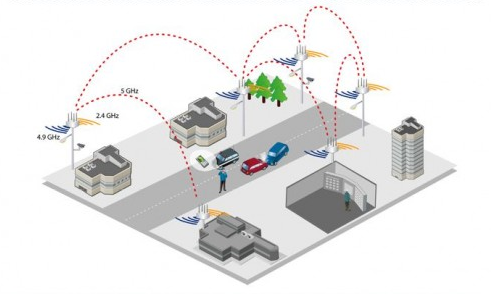
\includegraphics[width=\textwidth]{title}
        \label{fig:tit}
        \end{figure}
        
        \vfill
        {\sc Self Study Report}

        \vspace*{1cm}
        Prepared by\\
        {\sc Satya Prahlada Sthita Prajna Kandarpa \\
        UW ID 20402024 $\vert$ Userid \textit{spspkand} \\ 
        4B Mechatronics Engineering \\
        31 December 2015}

        \end{center}
\end{titlepage}



\cleardoublepage % Ends the current page and causes all figures and tables that have so far appeared in the input to be printed.
% In a two-sided printing style, it also makes the next page a right-hand (odd-numbered) page, producing a blank page if necessary.

% Letter of Submittal%
\begin{flushleft}
    41 Pineslope Crescent\\
    Scarborough, Ontario, Canada\\
    M1E 4M5
    
    31 December 2015
    
    Professor William Melek,\\
    Director of Mechatronics Engineering\\
    Department of Mechanical and Mechatronics Engineering\\
    University of Waterloo\\
    Waterloo, Ontario\\
    N2L 3G1
    
    Dear Sir,

    This report, titled "Video encoding techniques for networked low power applications", was prepared as my 4B Work Report for the University of Waterloo. This report is in fulfillment of the course WKRPT 400. The purpose of this report is to evaluate standard video encoding techniques in the context of networked low power video sensor applications and compare their performance with novel encoding techniques developed for distributed sensor networks.
    
    I got exposed to some innovative and novel media processing techniques at a startup I worked at which helped pique my interest in audio visual media processing. This report intends to provide guidance and critical technical evaluation from a software performance perspective to anyone interested in developing low power sensor networks that integrate cameras, audio sensors and mobile communication devices. 

    The technical analysis conducted by me for this purpose incorporates machine learning techniques to evaluate the standard video encoding technologies to produce optimized encoding parameters that may match the aforementioned specialized distributed video codecs in terms of video transcoding performance. This analysis maybe useful to anyone who would like to avoid the high license costs for the specialized video codecs.  
    
    This report was written entirely by me and has not received any previous academic credit at this or any other institution. 

    Sincerely,\\
    Satya Prahlada Sthita Prajna Kandarpa\\
    ID 20402024\\
\end{flushleft}
\cleardoublepage

 

% T A B L E   O F   C O N T E N T S
% ---------------------------------
    \linespread{1.0}
    \pagestyle{plain}
    \setcounter{page}{2}
    \renewcommand\contentsname{Table of Contents}
    \tableofcontents
    \cleardoublepage
    \phantomsection
    %\newpage
    
    % L I S T   O F   T A B L E S
    % ---------------------------
    \addcontentsline{toc}{chapter}{List of Tables}
    \listoftables
    \cleardoublepage
    \phantomsection		% allows hyperref to link to the correct page
    \newpage
    
    % L I S T   O F   F I G U R E S
    % -----------------------------
    \addcontentsline{toc}{chapter}{List of Figures}
    \listoffigures
    \cleardoublepage
    \phantomsection		% allows hyperref to link to the correct page
    %\newpage
    
    % L I S T   O F   S Y M B O L S
    % -----------------------------
    % To include a Nomenclature section
    % \addcontentsline{toc}{chapter}{\textbf{Nomenclature}}
    % \renewcommand{\nomname}{Nomenclature}
    % \printglossary
    % \cleardoublepage
    % \phantomsection % allows hyperref to link to the correct page
    % \newpage
    

%----------------------------------------------------------------------
% MAIN BODY
%----------------------------------------------------------------------
% Because this is a short document, and to reduce the number of files
% needed for this template, the chapters are not separate
% documents as suggested above, but you get the idea. If they were
% separate documents, they would each start with the \chapter command, i.e, 
% do not contain \documentclass or \begin{document} and \end{document} commands.
\linespread{1.6}
% \pagestyle{main}
\chapter*{Summary}
\addcontentsline{toc}{chapter}{Summary}
    The main purpose of this report is to give broad insight into the current state of video encoding technologies for various applications. The report introduces the burgeoning world of low power video sensor networks and talks about their applications in fields such as crowd, traffic and home surveillance and audio visual media (from an artistic context). 

    The report then describes the computational capabilities available for low power video sensors by analyzing the technical specifications for one standard low power video camera with wireless capabilities, the Dakota Ultra-Low Power Day/Night Camera. These technical specifications are then used to come up with viable constraints for video processing benchmarks such as time taken to encode a frame, network bandwidth required for continuous transmission, latency and Quality of Experience (QoE). These constraints may also be thought of as targets for the video processing system to be implemented by a low power camera.

    The report then introduces standard video processing techniques from a very low level so that the reader may gain insight into the computations and algorithms that power and drive today's digital media driven world. This is done to give the reader enough background knowledge to properly evaluate the project. Specifically, the structural anatomy of a video (on disk, in memory and during transport), is provided. Then, standard video processing techniques are described, namely encoding, decoding, transcoding and network transport. The report dives pretty deep into mathematical and image processing concepts that power video processing, and thus, a basic knowledge of signal processing techniques and linear algebra is assumed. The mathematical theorems that govern data redundancy reduction and computationally efficient algorithm design are explained from a higher level as a lot of the math was beyond an undergrad engineering student's grasp.
    
    A comprehensive analysis of standard video processing techniques including encoding, decoding and transcoding is presented from the perspective of their applicability to a network distributed video collection system. The various protocols available that enable video transport over a network aren't covered in much detail, however. The aforementioned distributed system has a server that acts as the centralized repository of video streams from each of the video sensors in the network. The process occurs sequentially starting from the capture of raw frames by a physical sensor, to the raw frames being encoded to a bit-stream by a video codec, the transportation of this bit-stream over a network to the centralized server and the final processing task, which involves using multi-view coding techniques to generate a multi-dimensional representation of all the videos. 

    The standard video codec covered by this report is the ubiquitous H.264/HVC compression standard developed by the ITU-T Video Coding Experts Group (VCEG) together with the ISO/IEC JTC1 Moving Picture Experts Group (MPEG). It is one of the most widely used video standards with applications including Internet streaming, Blu-ray disks and HDTV broadcasts over satellite and cable networks. The advantages offered by this video codec include providing imperceptible quality loss at lower bitrates than other standards and perhaps, the most important one, its ability to integrate well with existing video encoding and transmission infrastructure across a wide range of applications. 

    The report then presents an overview of the technologies behind the new video encoding technique known as Distributed Video Coding (DVC). The main advantages offered by video codecs that implement DVC include offloading encoding complexity to the decoder, which, for the purposes of this report happens on the centralized server. DVC is very flexible in that it allows user configurable distribution of coding complexity between the encoder and decoder based on application requirements. An experimental video codec implemented by researchers, namely the PRISM codec, is presented and its performance, characterized by the results of a few research papers, is analyzed based on the objectives defined for the low power video sensor. 

    The report then analyses a publicly available dataset of the transcoding performance of a few thousand youtube videos. This dataset includes characteristics such as input codec, frame-rate, size and output codec, frame-rate, bitrate and most importantly, memory and cpu time taken to transcode the input video to output video. This dataset is used to train two classes of statistical regression models, namely linear regression and non-linear regression models, to be able to predict the cpu time and memory required for transcoding. The videos in the dataset use 4 different codecs - flv, h264, mpeg4 and vp6. The transcoding was performed using the most widely used open source audio/video processing library, FFmpeg.

    The non-linear regression models trained using the dataset include k-Nearest Neighbors (kNN), Neural Networks (NN), Model Averaged Neural Networks (avNNet) and Multivariate Adaptive Regression Splines (MARS). All of the analyses are implemented using the statistical programming language, R using the packages \textit{caret} and \textit{AppliedPredictiveModelling}. The results from all the models are evaluated using two metrics, namely $R^2$ and $\text{Root Mean Squared Error}$, which are the statistical performance metrics for regression models.

    It is to be noted that the transcoding performance in the youtube dataset was measured on a fairly standard server computer with a high amount of processing power. However, the rationale behind training multiple models using this dataset is to be able to predict transcoding times for standard codecs irrespective of the computational power of the machine on which the transcoding operation is being run. This was done since there was no way to measure the computational encoding performance on an actual low power video sensor.

    In conclusion, this report provides a trained neural network model for interested parties to use and test on their own datasets to be able to gain predictions tailored to the hardware being used to implement their low power video sensor networks. It also recommends that the model be re-trained using a bigger portion of the youtube dataset. This wasn't done on the first try because of the lack of computational power required to train these datasets.
\cleardoublepage
% Change page numbering back to Arabic numerals
\pagenumbering{arabic}

\chapter{Introduction}
    \section{Background}

        The deployment of high-speed, wired and wireless networks such as 802.16, 802.16a, and 802.11b/g and the explosion of digital camera equipped cellular phones has already provided basic infrastructure for supporting communications in high data-rate wireless video sensor networks. These networks can find their way into many real-time applications needing video-based active monitoring of telemetry data in such diverse indoor and outdoor environments as hospitals, hotels, parking lots, highways, airports, and international borders. Typical video sensor networks are made up of multiple cameras with varying degrees of spatially and temporally overlapping coverage, generating correlated signals that need to be processed, compressed, and exchanged in a loss-prone wireless environment to facilitate real-time decisions. However, the sheer volume of visual data involved, with video signals ranging from a few hundreds of kilobits per second to a few megabits per second and more, poses new and unique challenges. There are numerous challenges to be addressed in order to make the second generation of broadband enabled wireless sensor video networks to take hold.

        A broadband network of wireless video sensors is subjected to three principal constraints:
        \begin{enumerate}
            \item {Limited processing capabilities and diverse display resolutions due in part to inexpensive device designs and limited battery power. These call for lightweight signal processing and compression algorithms at the individual sensor nodes and an architecture that can adapt to the differing processing capabilities of the encoding and decoding nodes.}
            \item {Limited power/energy budget requiring careful management for maximizing network lifetime, the quality of the acquired data, and the accuracy of the decisions. Communication is often the dominant power-consuming activity. Power management requires efficient compression algorithms that maximize the power utilization per bit communicated and controlled dormancy cycles in inter-sensor communication that preclude frequent intersensor communication. This motivates the need for distributed coding and processing.}
            \item {Information loss that is endemic to the harsh, loss-prone, wireless communication environment. This calls for robust coding algorithms, communication and networking protocols, and architectures that are immune to single points of failure. It is important to proactively build in robustness considerations into the architectural foundation rather than as after-thought bandage fixes.}
        \end{enumerate}

        The technologies that can make this vision a reality are within the reach of the general consumer and before them, entrepreneurs and electronics enthusiasts who would like to drive this revolution. Motivated by the enormous impact these technologies could potentially have, a survey of the general state of video encoding technologies revealed a growing interest among the Research and Development community in the field of Distributed Video Coding. 

        With the above constraints, the traditional views of video coding and transmission as being confined to a downlink scenario (such as television broadcast or download from a video server) need to be relaxed. In the prevalent video coding architectures such as MPEG-x and H.26x, video encoding is the primary computationally intensive task with the complexity dominated by the motion-search operation. Conventional video decoding, on the other hand, has significantly lower complexity. This skewed, somewhat rigid, complexity compartmentalization conflicts with the heterogeneous processing capability requirements of video sensor networks where the encoding units might be able to do only “lightweight” processing but the relay or decoding units might be more capable. The prevalent video coding architectures are also built upon the principle of (deterministic) predictive coding from which they derive their compression efficiency. 

\chapter{Video Processing And Transport}
    
    \section{Anatomy of a video}
        Digital videos are ubiquitous in the era of endless streaming/download/playback services such as Youtube, Netflix and VLC.
        
        Digital video is an ordered sequence of digital images, known as frames, played in succession at a given rate, usually represented as a framerate (frames per second or\mtext{fps}). 
        
        \begin{figure}[!h]
            \centering
            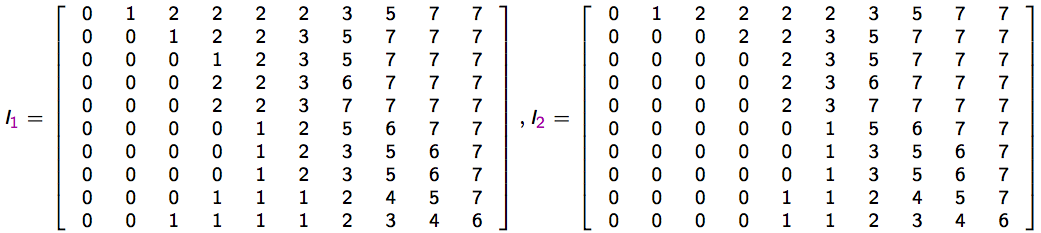
\includegraphics[width=\textwidth]{vidarch}
            \caption{Matrix representation of a video and its component frames}
            \label{vidarch}
        \end{figure}
        
        A grayscale video, represented by $V$, is a sequence of images $$ V = I_1, I_2, ... I_n, n = \text{number of frames in the video}$$, and $$I_k \mid k=1...n$$ is the matrix representation of an image of dimension $a \times b$. Please refer to Fig. \ref{vidarch} for a visual representation of the matrix images. Each image, $I_k$ consists of grayscale(brightness or intensity) values from a finite set $C$ of size $c$, where $$C = \{x \mid x = 0, 1, 2, ...N_c -1\}$$. A pixel is the basic unit of processing in images. Its location in a video maybe denoted by the 3-D co-ordinates 
        $$(k, m, n) \text{where } (k, m, n) = \text{(frame number, row number, column number)}$$
        
        \begin{figure}[!h]
            \centering
            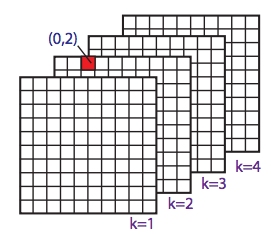
\includegraphics[width=0.5\textwidth]{framearch}
            \caption{Location of pixel $I_2(0,2)$ in a video frame}
            \label{framearch}
        \end{figure}
        
        The 3-D co-ordinates may also be represented by $I_k(m, n) \in C$. A visual representation of a pixel $I_2(0,2)$ is shown in Fig. \ref{framearch}\cite{Kundur}.
        
        Videos with color information use a similar representation with an additional color component. Pixels in color video frames may be represented by $$P(I_k, C_t, m, n )$$ where $C_t$ represents the color component numbered $t$. For example, an RGB image can have three possible values for t, i.e., $t \in (1, 2, 3)$. So, $P(I_k, C_t, m, n)$ represents the value of the color component $C_t$ for the pixel with frame co-ordinates $(m, n)$ and frame $I_k$ \cite{Lefevre2003}.

        Videos can be said to have two main representations in digital media - Pre-recorded videos and live/streamable videos. Disk based videos are playable files that may be stored on a personal computing device or a cloud server. These are binary representations of the video data, obtained by compressing raw video frames to achieve optimal spatiotemporal data representation, i.e., reduce redundant data in frames using a combination of motion tracking, Fourier or Discrete Cosine Transforms, Quantization and Variable Length Encoding \cite{Choupani}.
        \subsection{Pre-recorded Videos}
            Disk based video file formats may contain uncompressed video footage (RAW format) or encoded video footage (MP4, AVI, etc. formats). Most consumer focused video file formats consist of the following components:
            \subsubsection{Container}
                The container stores the video and/or audio data using separate encoding formats for video and audio. Popular container types include Matroska(MKV), FLV, Ogg, AVI, etc. It is to be noted that container selection constrains the available video encoding formats. The following table lists a few popular containers and their supported encoder formats.

                \begin{table}[!h]
                    \centering
                    \begin{tabular}{@{}|l|l|l|l|@{}}
                    \toprule
                    \rowcolor[HTML]{9B9B9B} 
                    Name             & File Extension & Container & Coding Formats                                                               \\ \midrule
                    MPEG-4(MP4)      & .mp4          & MPEG-4 Part 12  & H.264                                                                         \\ \midrule
                    Matroska         & .mkv           & Matroska  & Any                                                                                \\ \midrule
                    Flash Video(FLV) & .flv           & FLV       & H.264, VP6 \\ \bottomrule
                    \end{tabular}
                    \caption{Some common video containers and compatible video coding formats}
                    \label{my-label}
                \end{table}

            \subsubsection{Video coding(encoding) format}
                A video coding format (or sometimes video compression format) is a content representation format for storage or transmission of digital video content (such as in a data file or bitstream). Examples of video coding formats include MPEG-2 Part 2, MPEG-4 Part 2, H.264 (MPEG-4 Part 10), HEVC, Theora, Dirac, RealVideo RV40, VP8, and VP9.

        \subsection{Live/Streaming Videos}
            Streamable videos are defined as multimedia that is constantly received by and presented to an end user while being delivered by the provider. Streaming refers tot he delivery method of the video, rather than the video itself, and is an alternative to downloading a full video file. This report deals specifically with live streaming videos, which involves a source media type, a screen recorder in this case, an encoder to digitize the content, and a transport medium, usually one of HTTP, RTSP or RTP. 

            The main difference between downloadable and streamable videos is speed with which the end user may start watching the video. In case of downloadable videos (files), the user has to wait till the entire file has downloaded to be able to start playing the video. Streamable videos, however, make use of video codecs that are tailored to give the option of beginning playback from any position. They can make this happen by using multiple frame types, frame prediction methods. One frame type in particular, known as a keyframe, enables this resume capability of video from any position because of its decoupled nature from preceding and succeeding frames. Keyframes are implemented differently by video codecs but their essential function stays the same across all codecs. H.264, has a structure that enables interoperability during the video decode process with older video standards. The operational specifics of H.264 are explained in detail in Section \ref{sub:H.264}.

    \section{Video Processing}
        Video processing consists of three main processes - Encoding, Decoding and Transcoding
        \subsection{Encoding and Decoding}
            Encoding involves the analysis of uncompressed video files (RAW format) to remove redundant and/or visually indiscernible data and generate a bitstream representation of the video. This bitstream representation may then be used to generate files and/or streamable videos. Decoding involves recovering a playable (streamable) video from the bitstream generated by the encoding process. A \textit{video codec} is a program that can perform both encoding and decoding of a video or bitstream respectively. 
            \begin{figure}[!h]
                \centering
                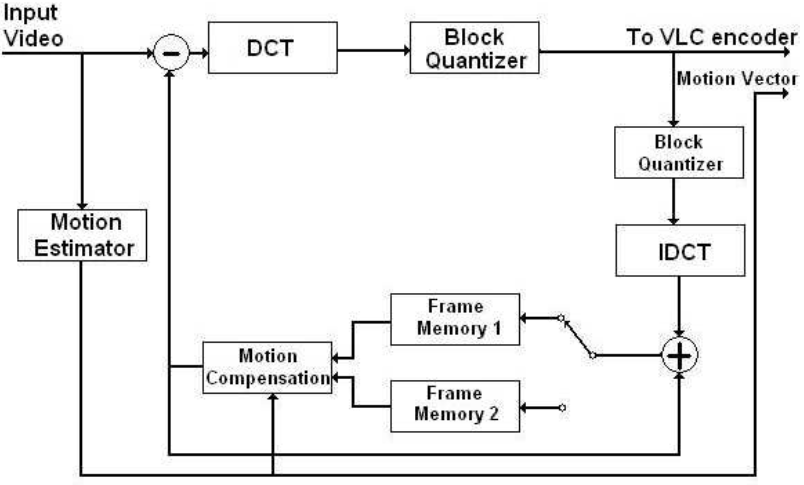
\includegraphics[width=\textwidth]{codec}
                \caption{Structure of a video codec}
                \label{codec}
            \end{figure}

            The general structure of a video codec is shown in Fig. \ref{codec}. It is important to note that the network transport stage of a streamable video involves sending this bitstream representation of a video to an end-user's browser or video playback application like VLC or Quicktime. Decoding occurs in the end-user application via available software or hardware codecs.
            \begin{figure}[!h]
                \centering
                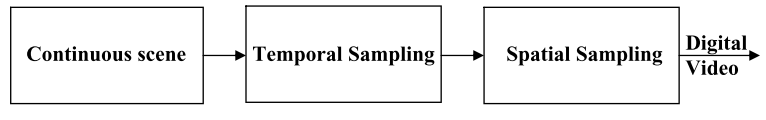
\includegraphics[width=\textwidth]{videnc}
                \caption{Digital video produced through compression techniques}
                \label{videnc}
            \end{figure}

            This process of data reduction is called video compression or encoding. When videos are captured by a camera, they are usually stored in an uncompressed format where each frame contains all the original data recorded by the capture device. This process is shown in Fig. \ref{videnc}. As evident in the figure, there are two sampling subprocesses, namely Spatial Sampling and Temporal Sampling, that are executed serially to produce a compressed video. 

            The data present in video frames can have 4 kinds of redundancies \cite{Saggi2010}.
            % \begin{itemize}
            %     \item {
            \subsubsection{Temporal Redundancy} % (fold)
            \label{sub:temporal_redundancy}
                Temporal Redundancy: Since the elapsed time between two consecutive frames is generally very short, consecutive frames tend to be very similar in content and thus, contain a lot of data redundancy. The differences between consecutive frames may be expressed by considering the displacements of objects in the frames and encoding this motion$'$s vectors and differences. 
                \begin{figure}[!h]
                    \centering
                    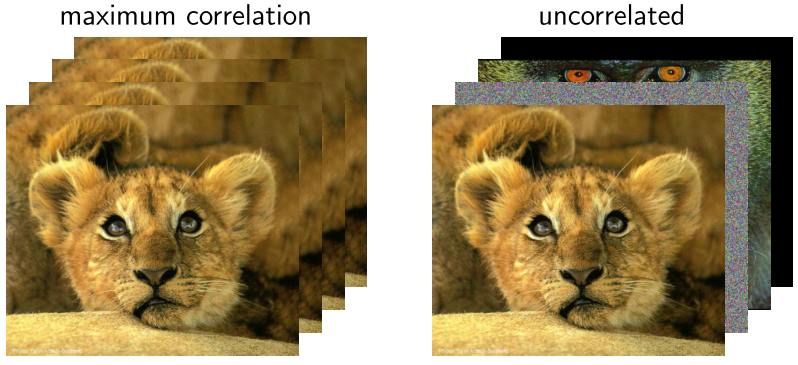
\includegraphics[width=0.8\textwidth]{tempredun}
                    \caption{Demonstration of temporal redundancy\cite{Kundur}}
                    \label{tempredun}
                \end{figure}

                To simplify this procedure, a frame is divided into small fixed (H-261, MPEG-1 encoders) or variable sized blocks(H.263, MPEG-4, H.264 encoders). Motion detection may then be performed by using a statistical measure to determine the best match for a block in a window centered at the block$'$s position in the second frame \cite{Choupani}.

            \subsubsection{Psycho Visual Redundancy} % (fold)
                \label{sub:psv_redundancy}  
                Psycho Visual Redundancy: Since the target audience for 99.99\% of all videos is a human recipient, the capabilities of the human visual system (HVS) need to be taken into account before encoding. The HVS is very sensitive to changes in luminance aka intensity compared to changed in chromaticity (color). In fact, the HVS is extremely good at inderring color details based on the intensity levels in an image. This knowledge maybe used to selectively subsample the color data in a frame while keeping the intensity data unchanged. 

                \begin{figure}[!h]
                    \centering
                    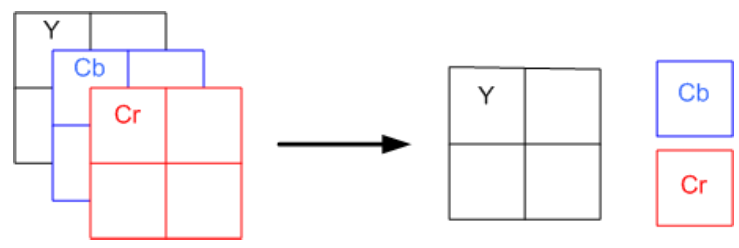
\includegraphics[width=0.8\textwidth]{psychredun}
                    \caption{Subsampling chromaticity to achieve data reducton\cite{Choupani}}
                    \label{psychredun}
                \end{figure}

                A frame maybe divided into macro blocks which are further divided into three layers with each layer holding one of the color components of the macroblock pixels. YCbCr is the color space used in almost all video coding standards because of its compatibility with the YUV color space used in most displays and televisions and its ability to separate chromaticity from intensity. If the macro block layer for each of Y, Cb and Cr components has 4 8x8 blocks, the Cb and Cr components can each be subsampled to 1 8x8 blocks. The format obtained in this way is referred to as 4:2:0 and the subsampling creates a data reduction of about 50\%. A macro block converted to 6 blocks of 8x8 each using 4:2:0 mode is shown in Fig. \ref{psychredun}
                % }
                % \item {
            \subsubsection{Spatial Redundancy} % (fold)
            \label{sub:spatial_redundancy}
                In any given frame, a pixel$'$s value is correlated to its neighboring pixel values most of the time. Thus, this value maybe predicted to a certain extent given the values of its neighboring pixels. An example is shown in Fig. \ref{spatredund}. High correlation means that pixels within a neighborhood have similar colors and zero correlation can mean that pixels in a neighborhood are unrelated in color.
                \begin{figure}[!h]
                    \centering
                    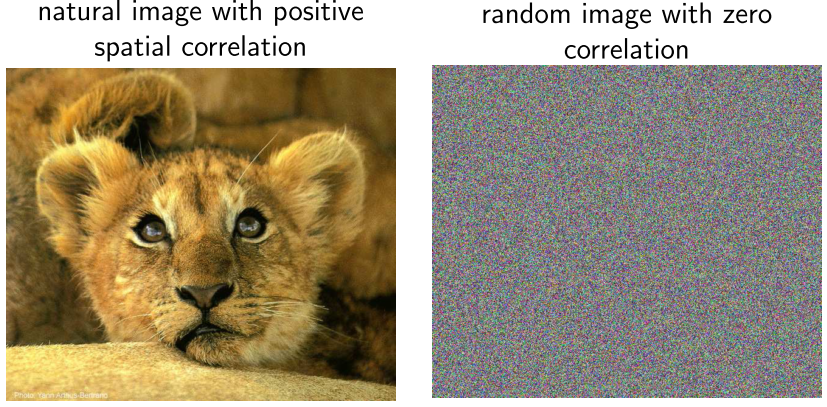
\includegraphics[width=0.8\textwidth]{spatredund}
                    \caption{Demonstration of spatial redundancy\cite{Kundur}}
                    \label{spatredund}
                \end{figure}
                Spatial redundancy may be reduced by using transforms such as Discrete Cosine Transform (DCT) or Discrete Wavelet Transform (DWT). These values are then quantized and converted to 1-D vectors by reading their values in zig-zag order. These transforms eliminate high frequency pixel values with low energy content. 

                The quality of the image/frame is directly related to this elimination, which means a trade-off between quality and compression ratio can be achieved based on constraints imposed by the transmission/playback medium of the video. A video meant to be consumed from disk based file systems can be allowed to retain more data during encoding while videos created for a streaming medium would need to take network bandwidth into consideration to determine an optimal compression ratio.

                In case of our application, the video is meant to recorded, encoded and sent over the network like a streamable video. So, higher compression ratios are desired while still being able to maintain video resolution and clarity rivaling HDMI (720p HD or 1280x720 frame dimensions).

                The process followed to achieve an optimum compression ratio is explained in later sections.

            \subsubsection{Statistical Redundancy}
                The process of reducing statistical redundancy is known as entropy coding. Entropy coding needs to occur after spatial redundancy reduction for optimum compression. The quantized frame data obtained after spatial redundancy reduction is then compressed by Run Length Encoding (RLE) and the resulting values are coded (each unique value gets a unique binary representation) using Huffman encoding. 

            \subsubsection{Live video considerations}
                Since temporal redundancy reduction makes use of the differences between consecutive frames, this may result in an accumulation of errors even if a frame experiences corruption during network transport. 

                This scenario can happen if the network transport method used is UDP (User Datagram Protocol), as UDP does not guarantee packet delivery and correct order of packet delivery as is the case with the TCP/IP protocol (used by HTTP). However, UDP is extremely useful for low latency data transmission due to its lack of error correction mechanisms that can guarantee packet delivery without corruption. The operational nature of UDP is commonly referred to as "send and forget".
                % \begin{figure}[!h]
                %     \centering
                %     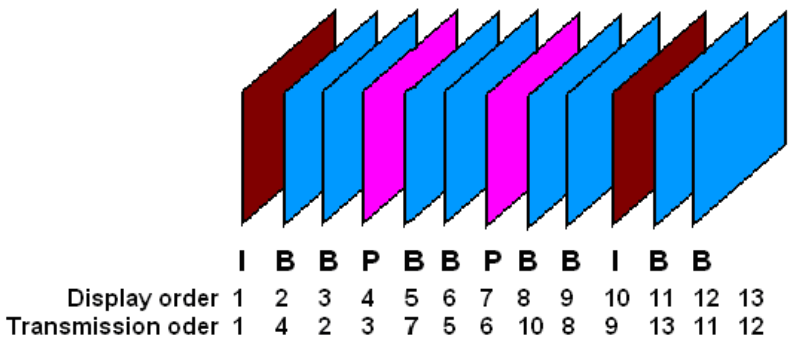
\includegraphics[width=0.8\textwidth]{frametypes}
                %     \caption{An example sequence of I, P and B frames in a video\cite{Choupani}}
                %     \label{frametypes}
                % \end{figure}

                Encoding methods that depend only on the previous frame create a serially accessible frame sequence that requires that the end user download and decode all frames before a particular frame to be able to correctly view the frame. This drawback has been overcome in various ways by different codecs. For example, the MPEG-2 codec uses multiple types of frames, with each type differentiated by the amount of data they hold and dependence on previous or future frames.

                % Special frame types called I-frames (Intra-coded frames), P-frames (Predicted picture) and B-frames (Bi-predictive frame) were invented to overcome this limitation and enable video playback from almost any seek position. An I-frame is an independent frame which is encoded without considering the previous frames. I-frames are also known as \textit{keyframes} and they are very similar to a static image file in that their decode process is completely independent of every other frame. A P-frame is a uni-directional difference frame obtained from either the previous I or P-frame. A B-frame encodes the difference between its previous and next P or I frames.\cite{Choupani}

                % I-frames are much bigger in size in comparision to P-frames and B-frames as they are completely independent of any frame. Thus, they cannot have any data redundancy reduction techniques applied to them during the encoding process. In terms of size taken up by each frame type, the following order is noticed:
                % $$ size(I-frame) > size(P-frame) > size(B-frame)$$
                % I-frames are the biggest, P-frames follow and B-frames have the least size and least data redundancy because of their ability to use frames before and after for data reference during decoding.

                Further improvements to video codecs resulted in the development of the H.264/AVC standard described in the following section. The performance and interoperability offered by the H/264 encoder absolutely blew every other encoder out of the water, especially for applications dependent on network transport.

        \subsection{H.264/AVC encoder}
        \label{sub:H.264}
            The H.264 encoder includes a set of improvements to the video coding process that provides enhanced compression performance relative to other encoders like MPEG-2 and VP6. The enhancements provided by H.264 specifically target broadcast, streaming, video telephony and other network friendly video representations. It provides significant improvement in rate distortion efficiency relative to existing standards \cite{Wiegand2003}. All of these features have enabled the H.264 codec to sort of become the de facto standard for video compression for network streaming applications. 

            \begin{figure}[!h]
                \centering
                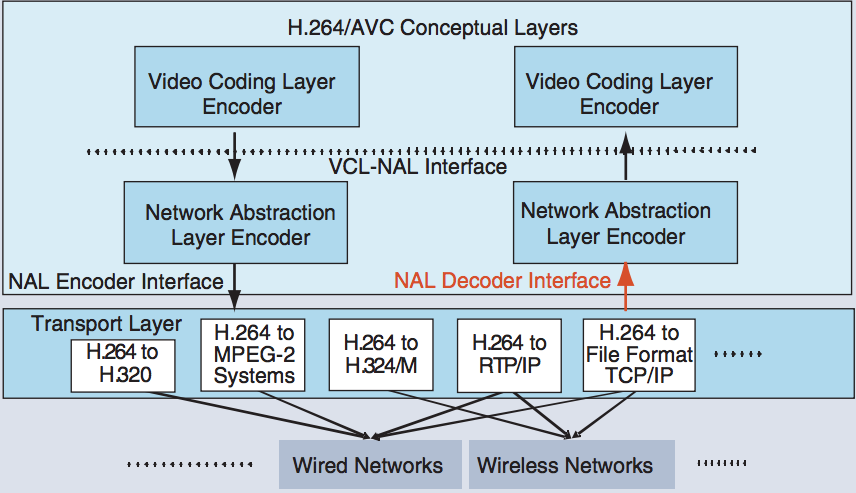
\includegraphics[width=0.8\textwidth]{h264struct}
                \caption{Structure of H.264/AVC encoder\cite{Ostermann2004}}
                \label{h264struct}
            \end{figure}

            A general architecture of the H.264/AVC codec is provided in Fig. \ref{h264struct}. For efficient transmission in different environments not only coding efficiency is relevant, but also the seamless and easy integration of the coded video into all current and future protocol and network architectures. This includes the public Internet with best effort delivery, as well as wireless networks expected to be a major application for the new video coding standard. The adaptation of the coded video representation or bitstream to different transport networks was typically defined in the systems specification in previous MPEG standards or separate standards like H.320 or H.324. However, only the close integration of network adaptation and video coding can bring the best possible performance of a video communication system. 

            Therefore H.264/AVC consists of two conceptual layers. The video coding layer (VCL) defines the efficient representation of the video, and the network adaptation layer (NAL) converts the VCL representation into a suitable format for specific transport layers or storage media. For circuit-switched transport like H.320, H.324M or MPEG-2, the NAL delivers the coded video as an ordered stream of bytes containing start codes such that these transport layers and the decoder can robustly and simply identify the structure of the bitstream. For packet switched networks like RTP/IP or TCP/IP, the NAL delivers the coded video in packets without these start codes \cite{Ostermann2004}.

            The following features describe the important features of the H.264 codec that make it a better choice over previous coding standards:
            \subsubsection {Intra Prediction}
                Intra prediction means that the samples of a macroblock in a frame (slice, in case of H.264) are predicted by using information of already transmitted macroblocks of the same frame. It is to be noted that each image is divided up into smaller packets (NALs) which can be read into macroblocks. H.264 uses varying modes for Intra Frame Prediction depending upon the rates of change of luminance and chromaticity in the image. 

            \subsubsection {Motion Compensated Prediction}
                This is a form of inter-frame (image) prediction. In this case, the macroblocks of an image can be predicted from already transmitted macroblocks of previous reference images. H.264 differs from previous standards (specifically, MPEG) in that it can use several preceding reference images for motion compensation prediction. For this purpose, an additional picture reference parameter has to be transmitted along with the standard motion displacement vectors usually needed for motion compensation prediction as described in Section \ref{sub:temporal_redundancy}.

            \subsubsection {Block Transform Coding}
                Former standards such as MPEG-1 and MPEG-2 used a Discrete Cosine Transform (DCT) with block size 8x8 for the purpose of transform coding. H.264 mainly uses 4x4 block sizes while switching to 2x2 blocks in special cases. It also uses 3 different kinds of applied integer transforms instead of a DCT. The first transform type of size 4x4 is applied to all samples of luminance and chromaticity components regardless of whether motion compensation prediction or intra prediction was applied. The other two types of transforms are Haddard transforms of sizes 4x4 and 2x2 respectively. 

                Compared to the DCT, the applied integer transforms used in H.264 have only integers between -2 and 2 in their transform matrix. This allows computing the transform and inverse transform in 16-bit arithmetic using only low complexity shift, add and subtract operations \cite{Ostermann2004}.

            \subsubsection {Entropy Coding Schemes}
                Entropy coding is used to reduce statistical redundancy, i.e., use lower number of bits to represet values that occur with high frequencies and a high number of bits to represent values that occur with low frequencies. This reduces the amount of data needed to represent the overall data required to make up the data.

        \subsection{Transcoding}
            Video transcoding refers to the process of data exchange between heterogeneous multimedia networks to reduce the complexity and transmission time by avoiding total decoding and re-encoding of a video bitstream. Despite the fact that a video stream is generated by eliminating all redundancies, many network channels may not have the necessary capabilities to handle these streams. This restriction may be overcome by reducing the video data size through a change in video format. In terms of video properties, this change can be affected by changing bits per pixel, pixels per frame (pixel density reduction), frames per second, video content or coding standard \cite{Choupani}.

            Video transcoding for real-time applications on raw video data is extremely time consuming because of the motion estimation and data transformation operations. Acceptable transcoding performance for real time operations can be achieved however, if the conversion of video formats is performed on compressed data rather than raw data. A few effective compressed data video transcoding techniques include:
            \begin{itemize}
                \item{Bitrate transcoding}
                \item{Spatial transcoding}
                \item{Temporal transcoding}
                \item{Standard transcoding}
            \end{itemize}
            A description of these techniques was deemed to be beyond the scope of this report, but more information may be found in the paper cited here \cite{Choupani}.

            In summary, it can be said that transcoding is something of an art form whereby one must balance dozens of requirements, formats, parameters and more. General video transcoding best practices are presented as follows:
            \begin{itemize}
                \item{Always encode for a specific quality rather than relying on bitrates. With bandwidth availability increasing across the board there is no need for using a target bitrate unless a specific limited device is being targeted (applicable to StremBox) or the quality required is unrealistic within bitrate constraints (in which case quality expectations have to be lowered)}
                \item{Avoid upscaling video dimensions from the original dimensions as this only blurs the video. In general, video players do automatic upscaling to make the video fit device screen, so it isn't necessary to do this during transcoding.}
                \item{Using Free and Open Source software like FFmpeg and libx264\cite{Video68:online} is highly recommended. These libraries have a community of video experts offering help and are very friendly. A lot of money may be saved by not using licensed and proprietary tools while still being able to provide insanely good video quality.}\cite{Trans44:online}
            \end{itemize}  

\chapter{Distributed Video Coding}
    \section{Overview}
        Distributed Video Coding (DVC) is ideally suitable to fulfill the above demand. DVC proposed a dramatic structural change to video coding by shifting the majority of complexity conventionally residing in the encoder towards the decoder by implementing distributed source coding concepts. The major task of exploiting the source redundancies to achieve the video compression is accordingly placed in the decoder. The DVC encoder thus performs a computationally very inexpensive operation enabling a significantly low cost implementation of the signal processor in DVC based video cameras\cite{Weerakkody2007}.
        
        \subsection{Slepian-Wolf (SW) Theorem}
            \begin{figure}[!h]
                \centering
                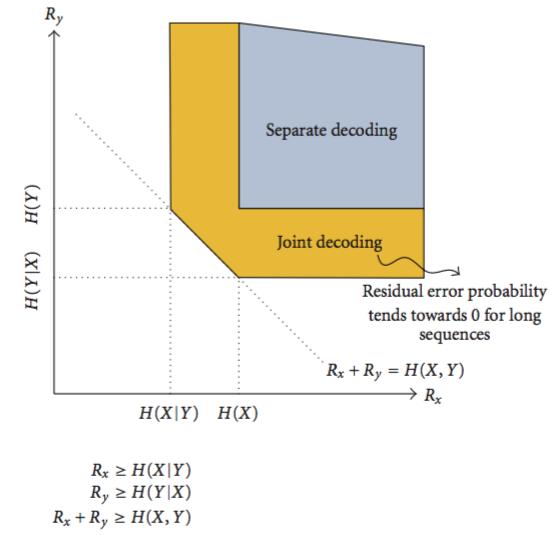
\includegraphics[width=0.5\textwidth]{swtheory}
                \caption{Achievable rates of lossless coding by distributed coding of two statistically dependent random signals\cite{Dufaux2009}}
                \label{swtheory}
            \end{figure}
            The SW theorem establishes some lower bounds on the achievable rates for the lossless coding of two or more correlated sources. More specifically, let us consider two statistically dependent random signals X and Y . In conventional coding, the two signals are jointly encoded and it is well known that the lower bound for the rate is given by the joint entropy H (X , Y ). Conversely, with distributed coding, these two signals are independently encoded but jointly decoded. In this case, the SW theorem proves that the minimum rate is still H (X , Y ) with a residual error probability which tends towards 0 for long sequences. Figure \ref{swtheory} illustrates the achievable rate region. In other words, SW coding allows the same coding efficiency to be asymptotically attained. However, in practice, finite block lengths have to be used. In this case, SW coding entails a coding efficiency loss compared to lossless source coding, and the loss can be sizeable depending on the block length and the source statistics.
        \subsection{Wyner-Ziv(WZ) Theory}
            Wyner and Ziv extended the Slepian-Wolf theorem by characterizing the achievable rate- distortion region for lossy coding with Side Information (SI). More specifically, WZ showed that there is no rate loss with respect to joint encoding and decoding of the two sources, under the assumptions that the sources are jointly Gaussian and an MSE distortion measure is used. This result has been shown to remain valid as long as the innovation between X and Y is Gaussian.

    \section{PRISM Encoder}
        \begin{figure}[!h]
            \centering
            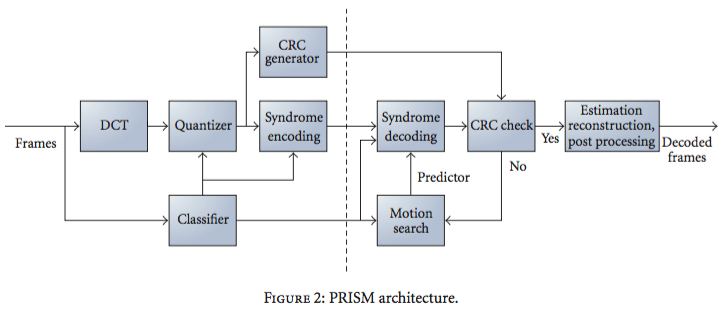
\includegraphics[width=\textwidth]{prism}
            \caption{Architecture of PRISM coding\cite{Dufaux2009}}
            \label{prism}
        \end{figure}
        PRISM, which stands for Power-efficient, Robust, hIgh compression Syndrome-based Multimedia coding, is one of the early practical implementations of DVC. This architecture is shown in Figure \ref{prism}. More specifically, each frame is split into 8 × 8 blocks which are DCT transformed. Concurrently, a zero-motion block difference is used to estimate their temporal correlation level. This information is used to classify blocks into 16 encoding classes. One class corresponds to blocks with very low correlation which are encoded using conventional Intra- coding. Another class is made of blocks which have very high correlation and are merely signaled as skipped. Finally, the remaining blocks are encoded based on distributed coding principles. More precisely, syndrome bits are computed from the least significant bits of the transform coefficients, where the number of least significant bits depends on the estimated correlation level. 

        The lower part of the least significant bit planes is entropy coded with a (run, depth, path, last) 4-tuple alphabet. The upper part of the least significant bit planes is coded using a coset channel code. For this purpose, a BCH code is used, as it performs well even with small block-lengths. Conversely, the most significant bits are assumed to be inferred from the block predictor or Side Information (SI). In parallel, a 16-bit Cyclic Redundancy Check (CRC) is also computed. At the decoder, the syndrome bits are then used to correct predictors, which are generated using different motion vectors. The CRC is used to confirm whether the decoding is successful.

\chapter{Machine Learning based Regression Model Training}
    \section{Dataset Characteristics}
        The dataset found at \cite{UCIM53:online} can be used to gain insight into characteristics of consumer videos found on UGC(Youtube). The features include bitrate, framerate, resolution, codec, number of i frames, number of p frames, number of b frames, size of i frames, size of p frames and size of b frames of the input video and the desired bitrate,framerate, resolution and codec of the output video which are given as a parameter to a transcoding service.

        \begin{figure}[!h]
            \centering
            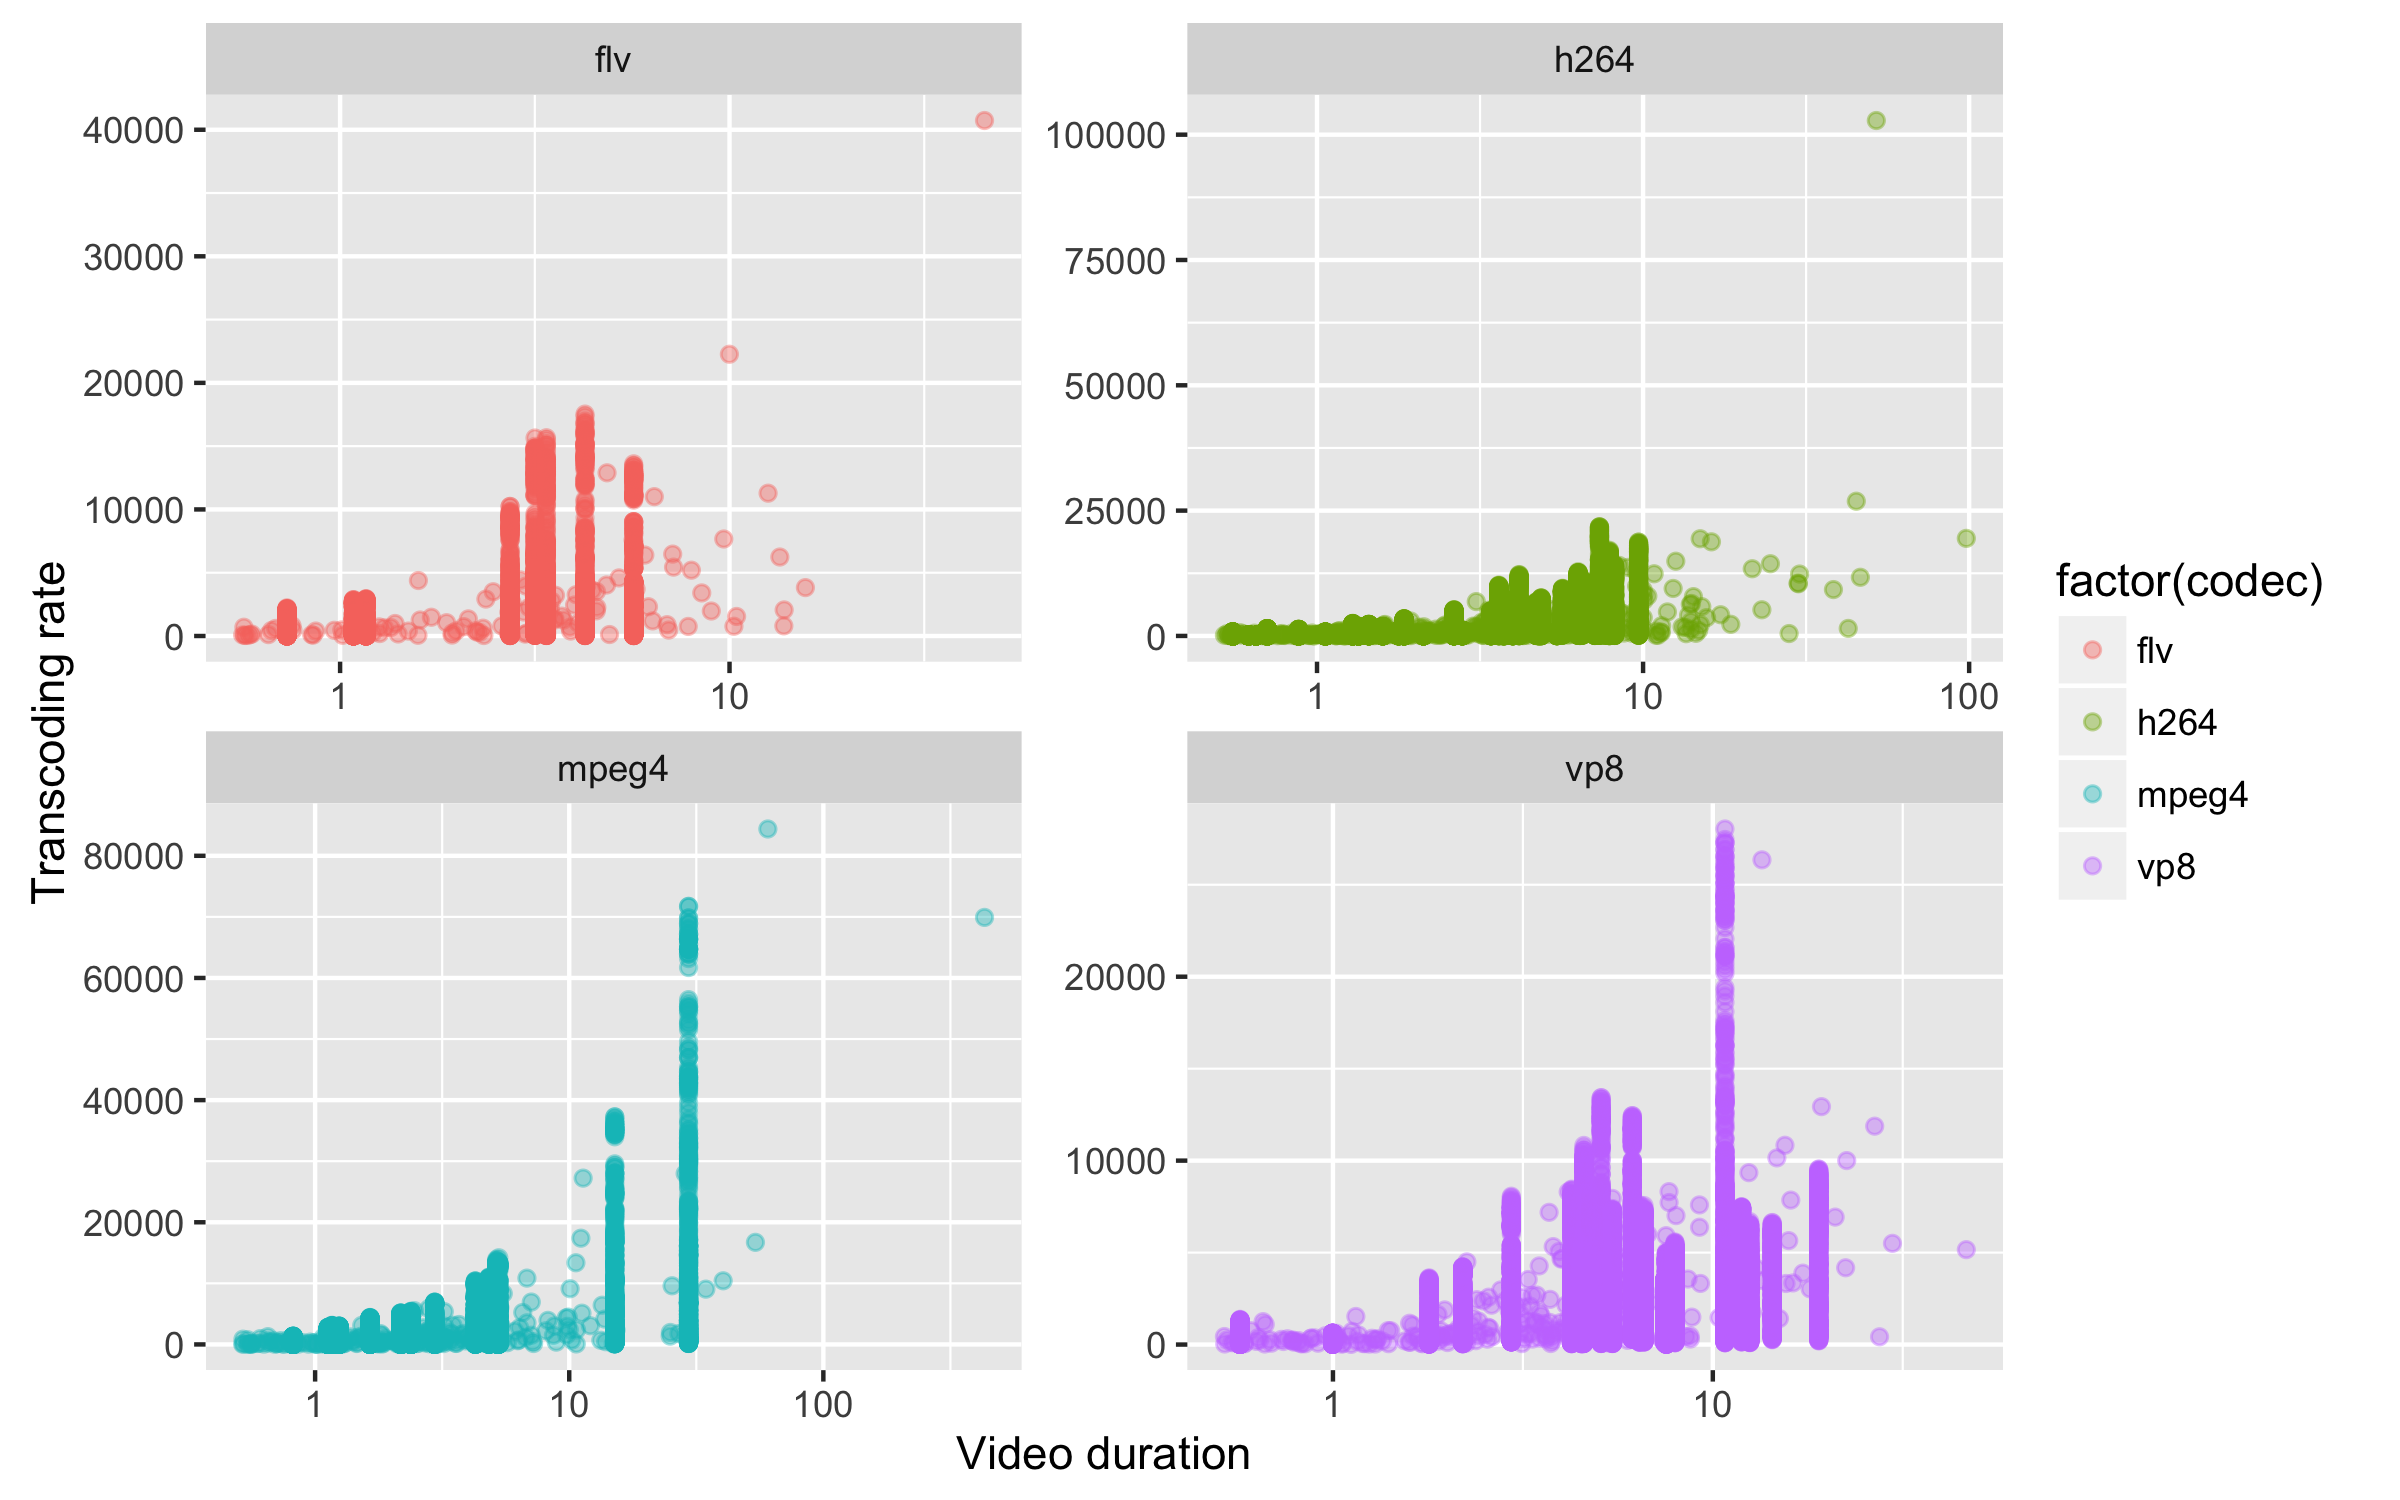
\includegraphics[width=\textwidth]{dur_vs_trate}
            \caption{Transcoding rate [fps] v/s video duration [min]}
            \label{dur_vs_trate}
        \end{figure}

        The second file of the dataset contains 20 columns(see column names for names) which include input and output video characteristics along with their transcoding time and memory resource requirements while transcoding videos to different but valid formats. The second dataset was collected based on experiments on an Intel i7-3720QM CPU through randomly picking two rows from the first dataset and using these as input and output parameters of a video transcoding application, ffmpeg.

        Please refer to Appendix \ref{app:ytvideo} for a thorough visualization based characterization of this dataset. A through exploration of this dataset, including scatterplots using the R package \textit{AppliedPredictiveModelling} \cite{apppredic}, threw up no single parameter as being primarily responsible for dictating the transcoding time of a video. This pointed towards the need for a machine learning based approach that can run through multiple regression models while tuning parameters in fine and small amounts to provide the best fit possible. The sheer number of input parameters to tune and account for to be able to predict one final output variable, the transcoding time, also led to the choice of using machine learning algorithms for prediction purposes.

    \section {Methodology for Regression based training}
        The use of complex classification and regression models is becoming more and more commonplace in science, finance and a myriad of other domains. Regression is concerned with modeling the relationship between variables that is iteratively refined using a measure of error in the predictions made by the model. Regression methods are a workhorse of statistics and have been cooped into statistical machine learning. This may be confusing because one can use regression to refer to the class of problem and the class of algorithm. Really, regression is a process.

        Mathematically, we can define the process of Regression modeling as follows. Suppose, we have an output $Y$ and a series of inputs or predictors (usually assumed to be independent variables). $$X_1, X_2, ...... X_n$$
        Then, the goals of a regression model are multiple:
        \begin{enumerate}
            \item {examine the relationship between inputs and outputs -- Do they tend to vary together? What does the “structure” of the relationship look like? Which inputs are “important”?}
            \item{ Given a new set of predictor values $X^{*}_1,...X^{*}_p$, what can be said about an unseen $Y^{*}$?}
            \item { Regression tools often serve as a building block for more advanced methodologies - Smoothing by local polynomials, for example, involves fitting lots of regression models "locally", while iteratively fitting weighted regressions is at the heart of the standard computations for generalized linear models}
        \end{enumerate}
        Machine learning is a subfield of computer science that evolved from the study of pattern recognition and computational learning theory in artificial intelligence. Machine learning explores the study and construction of algorithms that can learn from and make predictions on data. Such algorithms operate by building a model from example inputs in order to make data-driven predictions or decisions, rather than following strictly static program instructions.

        Regression analysis is widely used for prediction and forecasting, where its use has substantial overlap with the field of machine learning. Regression analysis is also used to understand which among the independent variables are related to the dependent variable, and to explore the forms of these relationships. In restricted circumstances, regression analysis can be used to infer causal relationships between the independent and dependent variables. However this can lead to illusions or false relationships, so caution is advisable; for example, correlation does not imply causation. In a narrower sense, regression may refer specifically to the estimation of continuous response variables, as opposed to the discrete response variables used in classification. The case of a continuous output variable may be more specifically referred to as metric regression to distinguish it from related problems.
        \clearpage
        
    \section {Evaluation of Software Packages}
        Two software library ecosystems were evaluated for the implementation of the regression based model training. It can be said that the ecosystem of packages and maturity is pretty good across all the platforms due to the explosion in popularity of machine learning techniques across all domains.
        \subsection {Python - \textit{scikit-learn}}
            The scikit-learn project provides an open source machine learning library for the Python programming language. The ambition of the project is to provide efficient and well-established machine learning tools within a programming environment that is accessible to non-machine learning experts and reusable in various scientific areas. The project is not a novel domain-specific language, but a library that provides machine learning idioms to a general purpose high-level language. Among other things, it includes classical learning algorithms, model evaluation and selection tools, as well as preprocessing procedures.

            All objects within scikit-learn share a uniform common basic API consisting of three complementary interfaces: an estimator interface for building and fitting models, a predictor interface for making predictions and a transformer interface for converting data \cite{scikit-learn}.

        \subsection {R - \textit{caret}}
            The caret package, short for classification and regression training, was built with several goals in mind:
            \begin{enumerate}
                \item{to eliminate syntactical differences between many of the functions for building and predicting models,}
                \item{to develop a set of semi-automated, reasonable approaches for optimizing the values of the tuning parameters for many of these models and}
                \item{create a package that can easily be extended to parallel processing systems.}
            \end{enumerate}
            The package contains functionality useful in the beginning stages of a project (e.g., data splitting and pre-processing), as well as unsupervised feature selection routines and methods to tune models using resampling that helps diagnose over-fitting. \textit{caret} depends on over 25 other packages, although many of these are listed as "suggested" packages which are not automatically loaded when caret is started. Packages are loaded individually when a model is trained or predicted.

        The author of this report had invested a lot of time in the past year in learning and getting familiar with the R ecosystem, through his work at another startup that dealt primarily with data analytics for realtime embedded communication systems, \href{http://acerta.ca}{Acerta Analytics}. Thus, it was decided to go ahead and use R, the \textit{caret \cite{caretR}} package for regression modelling, \textit{lattice \cite{latticebook}} and \textit{ggplot2 \cite{ggplot2}} for visualizations. This decision helped save a lot of time and enabled the entire machine learning portion of this report to be complete in 4 days.

    \section {Regression Training using \textit{caret}}
        \textit{Caret} has built in methods and and objects to deal with a data set from the first step of analysis, ie., exploratory data analysis to analyze, determine and mark the predictors and the output variables that need prediction. For example, the \textit{featurePlot} function may be used to plot each of the predictor variables against each other and mainly, the output variable. This can help one understand and determine right away, the presence of any linear correlations between the predictor variables and output variable. The plots that the \textit{featurePlot} function can handle include scatterplots, overlayed density plots,  box plots that show the extent of linear correlation and scatter plots with overlayed regression line smoothers. The official documentation available at \cite{Visua58:online} explains and shows a few example plots that help one understand the dataset. 

        In case of the youtube dataset, the number of predictor variables was found to be 18 and the output variables measured were the memory used for transcoding, \textit{umem} and the CPU time taken for the transcoding process, \textit{utime}. A summary of the elements present inside a data frame (standard R object) is presented below:

        \subsection{Data pre-processing and Splitting}
            As is evident in the summary presented above, a couple of new columns were added to convert the categorical variables for input and output codecs to integer factors. This had to be done since a few of the models being trained using the dataset are sensitive to the presence of categorical variables and are not really meant to be used with such data frame columns. An example of this can be seen in implementations of the k-Nearest Neighbors algorithm. This may be overcome by using Hamming distance instead of Euclidean distance for calculating distance between neighbors in the algorithm \cite{KnnW0:online}.

            An other addition to the dataset was the creation of a \textit{trans\_ rate} column, which stands for transcoding rate and was calculated with the following formula:
            $$transcoding rate =  \frac{Num. of frames}{Transcoding CPU time}$$

            This has been done to ensure that the output variable being modeled for is independent of the video size, and thus, can be closer to a good measure of the case where transcoding happens in real-time, aka streaming. 

            However, the most efficient way of determining the process of sample utilization, according to statistics, requires the usage of all the samples for training a model. Usually, this would result in a model over-fitting for the sample data. However, there are a few techniques that may be used to ensure over-fitting or under-fitting of data does not occur. These techniques, a few of which are cross-validation, bootstrapping, n-fold cross-validation and re-sampling \cite{Kuhn2008}.

            In the field of statistical data analysis, one of the first tasks is to determine how much of the finite dataset is to be used for model training while ensuring a certain portion of the dataset is kept aside for testing the efficacy of the model after training. Thus, it is important to ensure that a model being trained never gets exposed to the split testing /validation dataset. This is a very good measure of determining how well the model would perform when being used in real life. The main function of the test split dataset is to compare and evaluate performance across models, as a lot of statistical models are actually combinations of localized models.

            The \textit{caret} package, specifically has a \textit{createDataPartition} function, that analyses a dataset's characteristics such as multivariate correlation and determines the most randomized way to split the dataset. For regression, the function determines the quartiles of the data set and samples within those groups. The youtube dataset, which consists of about 69000 rows of data, would cause most models to take a lot of time to train with the computing resources available to this student. Thus, 5\% of the dataset was randomly sampled to be used as the training data. The rest of the 95\% of the dataset was then used to evaluate the performance of the models. A convenience function provided by \textit{caret}, \textit{nearZeroVar} was then used to determine a few non useful predictor variables and these were excluded from the predictors for testing and training datasets. These so-called near zero-variance predictors can cause problems during resampling for some models such as linear regression \cite{Kuhn2008}.

            This concludes the data pre-processing portion of this analysis. The function used by \textit{caret} to train using a model, the \textit{train} function, takes a \textit{preProc} argument that can be used to center and scale predictor variables, as required by models such as neural networks.
        \subsection{Tuning and building models}
            \begin{figure}[!h]
                \centering
                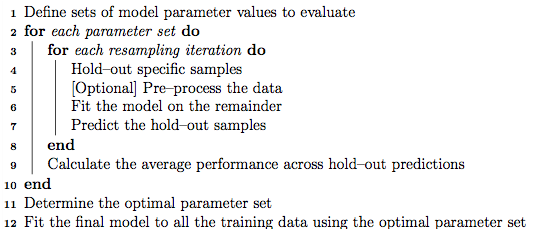
\includegraphics[width=0.8\textwidth]{training}
                \caption{Standard operating procedure to tune a model's parameters \cite{Model99:online}}
                \label{training}
            \end{figure}

            The general process that needs to be followed to do efficient parameter tuning while building a model is shown in Figure. \ref{training}. The \textit{caret} package has several functions that streamline the process of model building, tuning and evaluation. The \textit{train} function can be used to 
            \begin{itemize}
                \item {Evaluate, using resampling the effects of model parameter tuning on performance}
                \item {Choose the optimal model across these parameters}
                \item{Estimate model performance from a training set}\cite{Model99:online}
            \end{itemize}
            
            The models trained the youtube dataset were the following:
                \paragraph{k-Nearest Neightbors}
                    k-Nearest Neighbors (kNN) is a non parametric lazy learning algorithm which defers the decision to generalize beyond the training samples till a new query is encountered. For regression, kNN may be used to estimate continuous variables. It works by using a weighted average of the k-nearest neighbors ,weighted by the inverse of their Euclidean or Manhattan distance.
                    \begin{itemize}

                    \item{Parameters and Evaluation metrics:} % (fold)

                        The parameters to tune in the kNN model is the number of nearest neighbors used to compute the distance from existing samples for a new sample, \textbf{k}.

                        kNN maybe evaluated using the Root Mean Squared Error, RMSE.
                    
                    \end{itemize}

                \paragraph{Neural Networks}
                    \begin{figure}[!h]
                        \centering
                        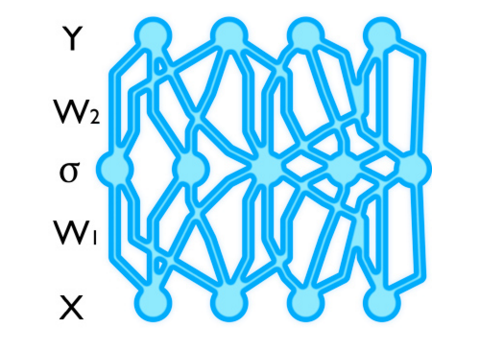
\includegraphics[width=0.4\textwidth]{anns}
                        \caption{A neural network (a deep learning tool) \cite{What93:online}}
                        \label{anns}
                    \end{figure}
                    Artificial Neural networks are computing systems made up of a number of simple, highly interconnected processing elements, which process information by their dynamic state response to external inputs. Neural networks are typically organized in layers. Layers are made up of a number of interconnected 'nodes' which contain an 'activation function'. Patterns are presented to the network via the 'input layer', which communicates to one or more 'hidden layers' where the actual processing is done via a system of weighted 'connections'. The hidden layers then link to an 'output layer' where the answer is output as shown in Figure \ref{anns}.
                    \begin{itemize}
                        \item{Parameters and Evaluation metrics:}
                            An ANN maybe described by two parameters, size and decay. Its performance can be evaluated using regression plots, and RMSE and the coefficient of determination, $R^2$, which is a measure of how well the model was able to predict each sample.
                    \end{itemize}

                \paragraph{Multiple Adaptive Regressive Splines (MARS)}
                    MARS is a form of regression analysis introduced by Jerome H. Friedman in 1991. It is a non-parametric regression technique and can be seen as an extension of linear models that automatically models nonlinearities and interactions between variables. The MARS model is a weighted sum of Basis functions, $$f(x) = \sum_{1=1}^{k}c_i B_i(x)$$ \cite{friedman1991multivariate}. $c_i$ is a constant coefficient. Each basis function can take three different forms - a constant, a hinge function and a product of two or more hinge functions.

                    MARS models may also be evaluated using the standard regression measures RMSE and the coefficient of determination, $R^2$

        \subsection {Resampling and Model Cross-Validation}
            Resampling is the process of creation of modified datasets from the training dataset. Each data set has a corresponding set of hold-out samples. For each candidate tuning parameter combination, a model is fit to each resampled data set and is used to predict the corresponding held out samples. The resampling performance is estimated by aggregating the results of each hold-out sample set. These performance estimates are used to evaluate which combination(s) of the tuning parameters are appropriate. Once the final tuning values are assigned, the final model is refit using the entire training set \cite{Kuhn2008}.

            For the \textit{train} function, the possible resampling methods are: bootstrapping, k-fold crossvalidation, leave-one-out cross-validation, and leave-group-out cross-validation (i.e., repeated splits without replacement). By default, 25 iterations of the bootstrap are used as the resampling scheme. ALll the models used for the youtube dataset training, used 10-fold cross-validation repeated 10 times to ensure proper fitting of sample data.

            The train function can also perform cross validation, this setting maybe configured in the tuneGrid and trainControl function arguments. Please refer to Appendix \ref{rcode} for the actual code that shows these parameters.
        \clearpage

    \section {Testing/Training Results}

        \subsection {Neural Network Models}
            \begin{figure*}[!ht]
            \begin{subfigure}[t]{0.5\textwidth}
                \centering
                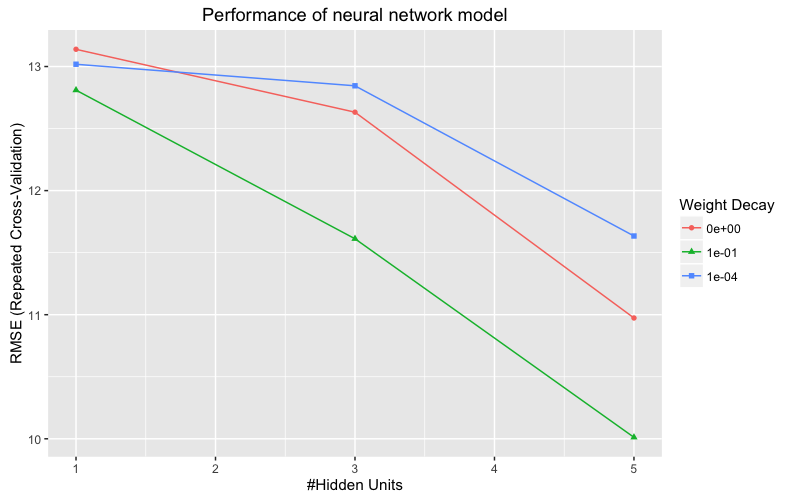
\includegraphics[width=1.1\textwidth]{nnetresults}
                \caption{Peformance Tuning}
                \label{nnetresults}
            \end{subfigure}%
                ~ 
            \begin{subfigure}[t]{0.5\textwidth}
                \centering
                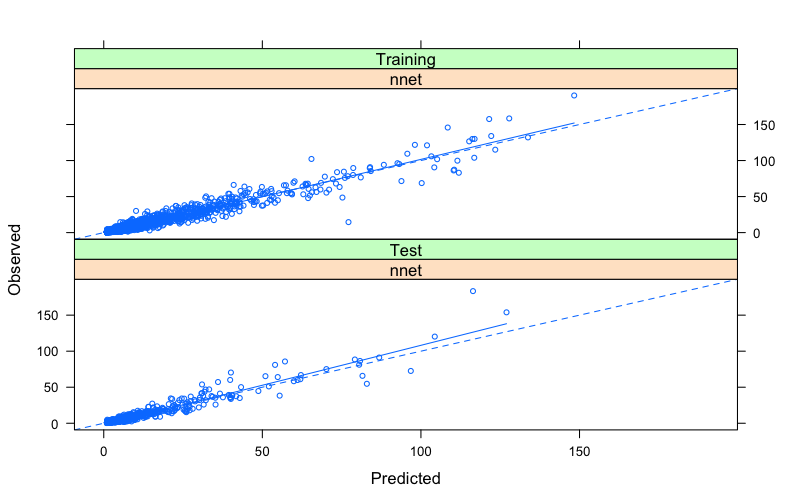
\includegraphics[width=1.1\textwidth]{nnet_pred_obs}
                \caption{Regression plot}
                \label{nnet_pred_obs}
            \end{subfigure}
            \caption{Neural Network Performance Metrics}
            \end{figure*}
            The neural network model performed exceptionally well in fitting both the training and test datasets to itself. This is evident in Fig. \ref{nnet_pred_obs}. Fig. \ref{nnetresults} shows how the RMSE changes as the number of hidden units in the neural network are increased. The best performance seems to have happened when using a decay of 0 and hidden unit size of 5. Please refer to Table \ref{RMSE} and Table \ref{Rsquared} for specific values of performance measures RMSE and $R_2$.
            \begin{figure*}[!ht]
            \begin{subfigure}[t]{0.5\textwidth}
                \centering
                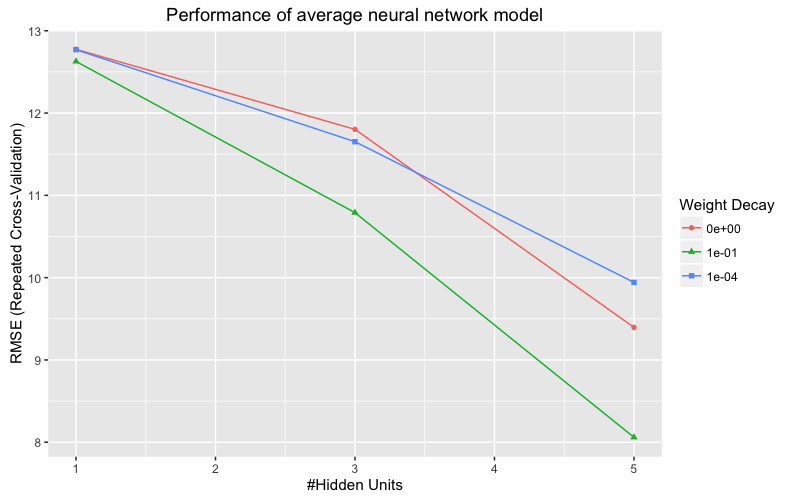
\includegraphics[width=1.1\textwidth]{avnnetresults}
                \caption{}
                \label{avnnetresults}
            \end{subfigure}%
                ~ 
            \begin{subfigure}[t]{0.5\textwidth}
                \centering
                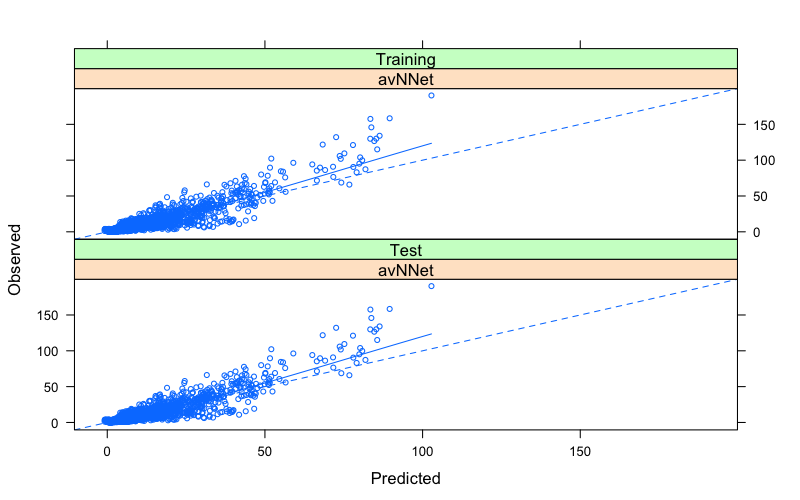
\includegraphics[width=1.1\textwidth]{avnnet_pred_obs}
                \caption{}
                \label{avnnet_pred_obs}
            \end{subfigure}
            \caption{avg Neural Network Performance Measures}
            \end{figure*}

            The averaged neural network performed slightly worse than a simple neural network on both the training and test datasets. THis may be noticeable because of the amount of variation from the regression line in Fig. \ref{avnnet_pred_obs}. Its best performance, when evaluated using the RMSE, seems to have happened with a weight decay parameter of 0.1. Please refer to Table \ref{RMSE} and Table \ref{Rsquared} for specific values of performance measures RMSE and $R^2$
        \subsection {Nearest Neighbor Models}
            \begin{figure*}[!ht]
            \begin{subfigure}[t]{0.5\textwidth}
                \centering
                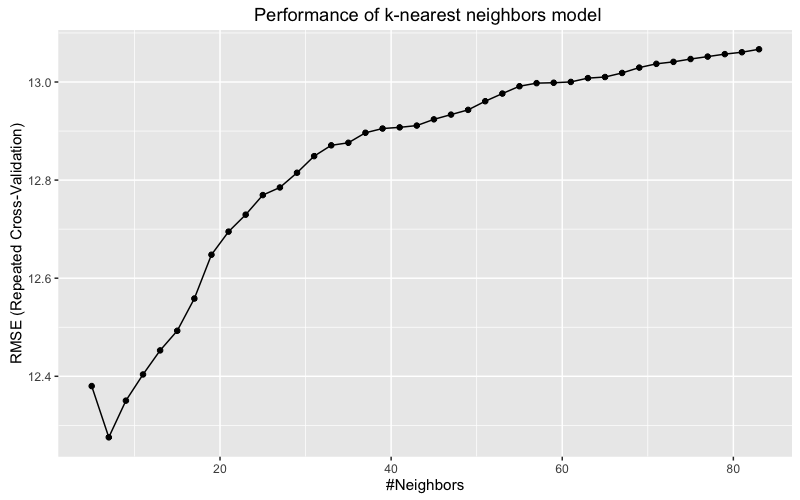
\includegraphics[width=1.1\textwidth]{knnresults}
                \caption{}
                \label{knnresults}
            \end{subfigure}%
                ~ 
            \begin{subfigure}[t]{0.5\textwidth}
                \centering
                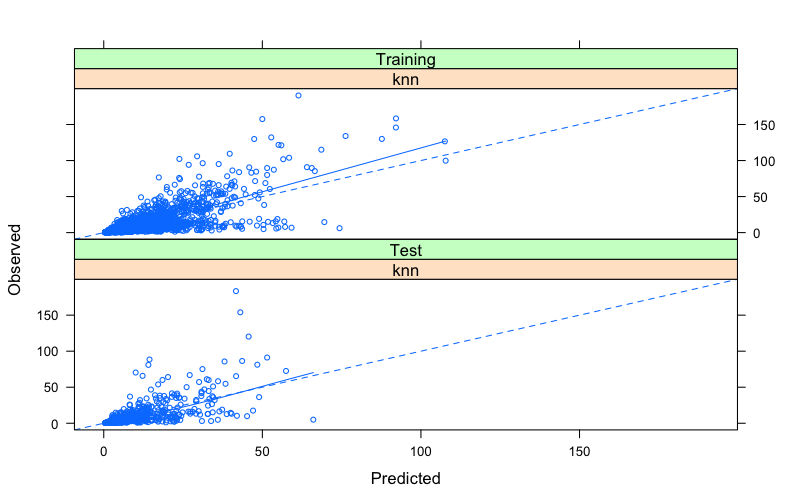
\includegraphics[width=1.1\textwidth]{knn_pred_obs}
                \caption{}
                \label{knn_pred_obs}
            \end{subfigure}
            \caption{kNN Performance Measures}
            \end{figure*}

            The performance of the k-Nearest Neighbor model decreased while k was increased till $k = 7$. Then its performance exponentially degraded as k increased further higher. Its regression plot, in Fig. \ref{knn_pred_obs}, also shows a lot of both the training and test samples having higher degree of error from the regression line. Please refer to Table \ref{RMSE} and Table \ref{Rsquared} for specific values of performance measures RMSE and $R^2$

        \subsection {Multivariate Adaptive Regression Splines}
            \begin{figure*}[!ht]
            \begin{subfigure}[t]{0.5\textwidth}
                \centering
                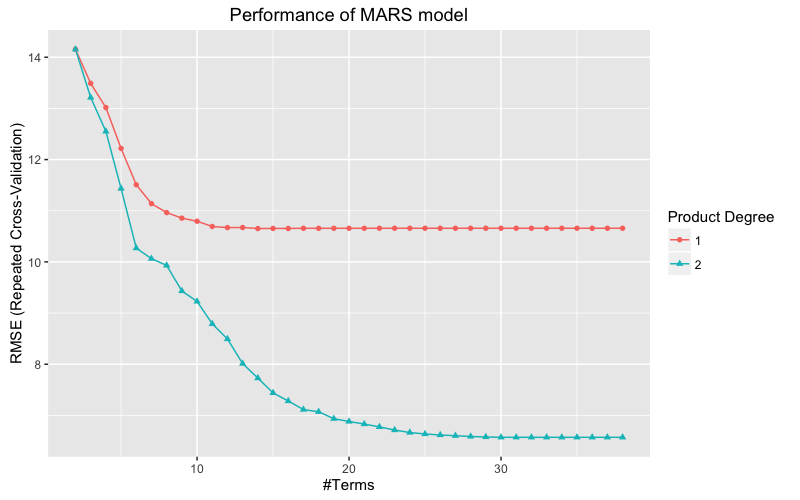
\includegraphics[width=1.1\textwidth]{marsresults}
                \caption{}
                \label{marsresults}
            \end{subfigure}%
                ~ 
            \begin{subfigure}[t]{0.5\textwidth}
                \centering
                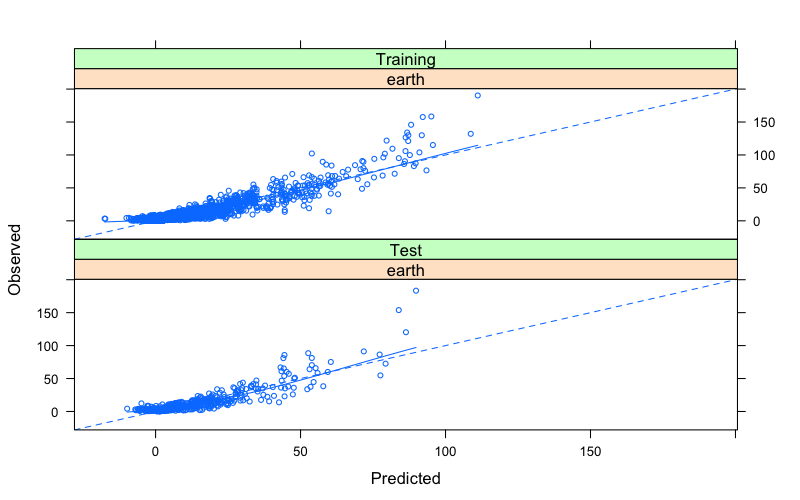
\includegraphics[width=1.1\textwidth]{mars_pred_obs}
                \caption{}
                \label{mars_pred_obs}
            \end{subfigure}
            \caption{MARS Performance Measures}
            \end{figure*}

            The performance of the MARS model almost rivals that of the neural network model. In fact, there is no way to differentiate between their regression fit without referring to $R^2$ values. Its performance increased exponentially when the number of basis functions was increased with the best performance deemed to have occurred with about 37 basis functions in the models. Please refer to Table \ref{RMSE} and Table \ref{Rsquared} for specific values of performance measures RMSE and $R^2$

        \subsection {Resampling Statistics}
            This section shows the variation of the performance measures Root MEan Squared Error (RMSE) and $R^2$ across different resamples of the training data. In summary, it maybe said that both the MARS neural network models. THe average neural network model seemed to show a more reliable and consistent RMSE and $R^2$ values across multiple resamples.
            \begin{table}[!hp]
                \begin{center}
                \begin{tabular}{lrrrrrrr}
                \hline\hline
                \multicolumn{1}{l}{Model}&\multicolumn{1}{c}{Min.}&\multicolumn{1}{c}{1st Qu.}&\multicolumn{1}{c}{Median}&\multicolumn{1}{c}{Mean}&\multicolumn{1}{c}{3rd Qu.}&\multicolumn{1}{c}{Max.}&\multicolumn{1}{c}{NA's}\tabularnewline
                \hline
                knn&$9.110$&$11.040$&$12.010$&$12.280$&$13.500$&$17.210$&$0$\tabularnewline
                mars&$4.833$&$ 5.883$&$ 6.360$&$ 6.572$&$ 7.393$&$ 9.972$&$0$\tabularnewline
                nnet&$3.661$&$ 6.532$&$10.680$&$10.010$&$13.260$&$17.210$&$0$\tabularnewline
                avnnet&$4.177$&$ 6.298$&$ 7.465$&$ 8.060$&$ 9.353$&$13.460$&$0$\tabularnewline
                \hline
                \end{tabular}\end{center}
                \caption{RMSE\label{RMSE}} 
                \end{table}
                %latex.default(object = object[[i]], caption = nx[i], label = nx[i],     append = file != "", title = title, file = file, caption.lot = NULL,     caption.loc = caption.loc, ...)%
                \begin{table}[!hp]
                \begin{center}
                \begin{tabular}{lrrrrrrr}
                \hline\hline
                \multicolumn{1}{l}{Model}&\multicolumn{1}{c}{Min.}&\multicolumn{1}{c}{1st Qu.}&\multicolumn{1}{c}{Median}&\multicolumn{1}{c}{Mean}&\multicolumn{1}{c}{3rd Qu.}&\multicolumn{1}{c}{Max.}&\multicolumn{1}{c}{NA's}\tabularnewline
                \hline
                knn&$0.2175$&$0.3784$&$0.4366$&$0.4321$&$0.4907$&$0.6384$&$0$\tabularnewline
                mars&$0.7477$&$0.8197$&$0.8435$&$0.8389$&$0.8585$&$0.8990$&$0$\tabularnewline
                nnet&$0.2102$&$0.3626$&$0.4736$&$0.5857$&$0.8351$&$0.9568$&$0$\tabularnewline
                avnnet&$0.2547$&$0.6865$&$0.8000$&$0.7541$&$0.8544$&$0.9396$&$0$\tabularnewline
                \hline
                \end{tabular}
                \caption{$R^2$\label{Rsquared}} 
                \end{center}
                \end{table}
        \subsection {Resampling Visualizations}
            \begin{figure}[!h]
                \centering
                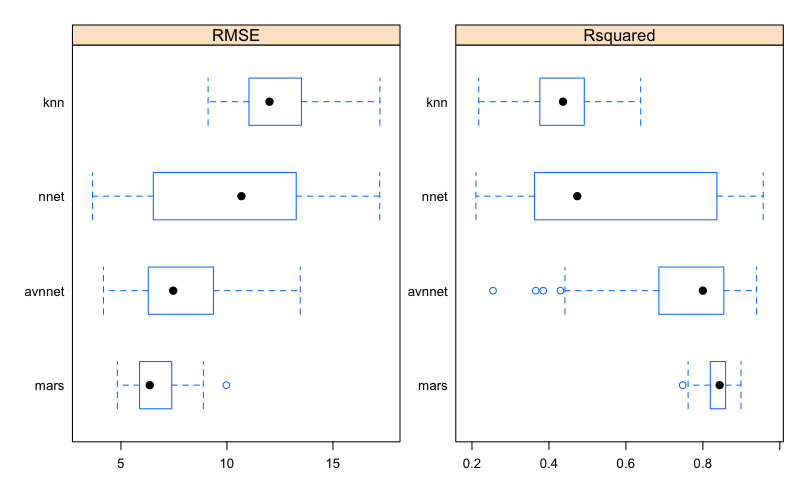
\includegraphics[width=\textwidth]{resamp_bwplot}
                \caption{Box whisker plot of RMSE and $R^2$ variation across resamples}
                \label{resamp_bwplot}
            \end{figure}
            Figures. \ref{resamp_bwplot} and \ref{resamp_dotplot} are visual representation of the data presented in Table \ref{RMSE}. Once again, the MARS model is deemed to be the most consistent model because of its low variation of RMSE and $R^2$ values across resamples. These plots make it very clear that the MARS model fit the training data consistently.
            
            \begin{figure}[!h]
                \centering
                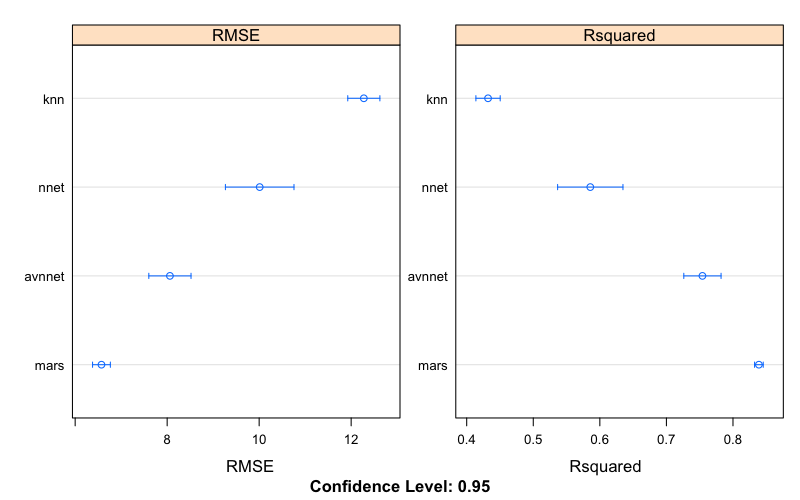
\includegraphics[width=\textwidth]{resamp_dotplot}
                \caption{Dot plot of RMSE and $R^2$ variation across resamples}
                \label{resamp_dotplot}
            \end{figure}

            \begin{figure}[!h]
                \centering
                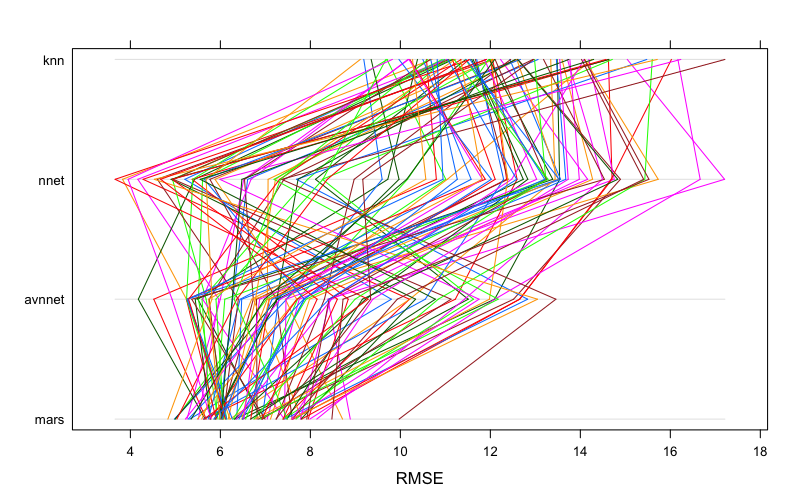
\includegraphics[width=\textwidth]{resamp_parallelplot}
                \caption{Parallel plot of RMSE and $R^2$ variation across resamples}
                \label{resamp_parallelplot}
            \end{figure}
            Figure \ref{resamp_parallelplot} shows how the RMSE varied for each model across resamp runs. Please note that this is a measure of cross-validation across models for each resample of the training data set. This maybe achieved by using \textit{caret's} \textit{resamples} function that takes in a list of trained models and a training dataset and a number of iterations of the resample process. All the relevant code for producing this cross-model resampling and visualization is also available in Appendix \ref{rcode} towards the end.

    \section{Statistical Performance Measures}

        \subsection {Performance evaluation}
            \begin{table}[!hp]
                \begin{center}
                \begin{tabular}{lrr}
                \hline\hline
                \multicolumn{1}{l}{Model}&\multicolumn{1}{c}{rmse}&\multicolumn{1}{c}{r2}\tabularnewline
                \hline
                KNN&$10.59699280697047$&$0.584605561041047$\tabularnewline
                AvgNN&$ 6.95034584039986$&$0.843654549692612$\tabularnewline
                MARS&$ 6.29845637084742$&$0.850651878271596$\tabularnewline
                NN&$ 4.01016583316771$&$0.939547289034280$\tabularnewline
                \hline
                \end{tabular}
                \caption{Results of model performance on trained dataset}
                \label{train-res}
                \end{center}

            \end{table}
            Table \ref{train-res} shows the best case performance of each model on the training dataset. The neural network comes out on top when evaluated using this data only. MARS comes behind in a close second place. 

            \begin{table}[!hp]
                \begin{center}
                \begin{tabular}{lrr}
                \hline\hline
                \multicolumn{1}{l}{Model}&\multicolumn{1}{c}{rmse}&\multicolumn{1}{c}{r2}\tabularnewline
                \hline
                KNN&$12.44409507063652$&$0.403246960924018$\tabularnewline
                AvgNN&$ 8.21448372643189$&$0.764592868929468$\tabularnewline
                MARS&$ 6.86267500478760$&$0.818602643604257$\tabularnewline
                NN&$ 4.81454518621358$&$0.911059846936685$\tabularnewline
                \hline
                \end{tabular}
                \caption{Results of model performance on the complete dataset}
                \label{test-res}
                \end{center}
            \end{table}
            Table \ref{test-res} shows the best case performance of each model on the test data set. This table is arguably a lot more important for performance evaluation as it eliminates the possibilities of over fitted models, etc. Once again, the neural network ended with a performance very similar to its performance on the training dataset. COnsidering that the training set was only 5\% of the total dataset, this performance is actually extremely good. The MARS model, on the other hand, seems to have faltered on the test dataset as its $R^2$ value decreased slightly and the RMSE values increased by a tiny bit. In terms of RMSE however, The NN model comes out on top again with an RMSE value of 4.84. 
        \subsection {Variable Importance}
            \begin{figure*}[!ht]
            \begin{subfigure}[t]{0.5\textwidth}
                \centering
                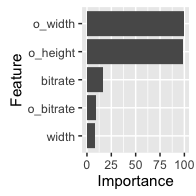
\includegraphics[height=5cm]{avnnetvarimp}
                \caption{avgNNet Important Predictors}
                \label{avnnetvarimp}
            \end{subfigure}%
                ~ 
            \begin{subfigure}[t]{0.5\textwidth}
                \centering
                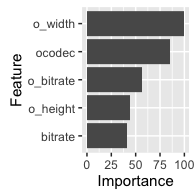
\includegraphics[height=5cm]{marsvarimp}
                \caption{MARS Important Predictors}
                \label{marsvarimp}
            \end{subfigure}
            \end{figure*}
            \begin{figure*}[!ht]
            \begin{subfigure}[t]{0.5\textwidth}
                \centering
                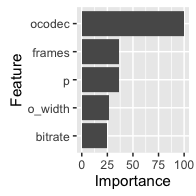
\includegraphics[height=5cm]{nnetvarimp}
                \caption{NNet Important Predictors}
                \label{nnetvarimp}
            \end{subfigure}%
                ~ 
            \begin{subfigure}[t]{0.5\textwidth}
                \centering
                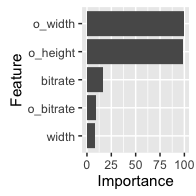
\includegraphics[height=5cm]{knnvarimp}
                \caption{K-Nearest neighbors important predictors}
                \label{knnvarimp}
            \end{subfigure}
            \caption{Top Predictors for Each Model}
            \end{figure*}
            This section intends to show the importance of the non-applicability of linear models to complex datasets like the youtube dataset where the number of predictors are very high with complex inter-predictor relationships.

    % \section{}
\chapter{Conclusions and Recommendations}
    \section{Conclusions}
        In conclusion, it is recommended that one use the neural network model file available at the Github repository for this report, cited here \cite{prajn0:online}. This file maybe loaded into an R environment using the $load(filename)$ function call and new datasets maybe used to gain predictions of 
    \section{Recommendations}
        It is recommended that the models be re-trained using additional computational power and a much bigger portion of the youtube dataset. Even though the models generated got a pretty good fit, the amount of time taken to train each model was extremely high for the hardware available for the author, a paltry Macbook Air 13" with no GPU processing power. It is also recommended that the youtube dataset be used to train a Support Vector Machine dataset in hopes of gaining a better fitting model.

\appendix
\chapter{Appendix}
    \section{Programming Code}
        \label{rcode}
        All the code used to generate the visualizations for this report can be found in the github repository located at \href{https://github.com/prajnak/machine_learning_experiments}{Github}.
        \subsection {Model Training and Results Visualization - models.R}
        \begin{multicols}{2}
        \begin{minted}[autogobble, breaklines, fontsize=\tiny]{R}
            # Multiple training routines EPage 82
            save_plots = T
            library(caret)
            library(AppliedPredictiveModeling)
            library(dplyr)
            library(lattice)
            set.seed(0)
            #load('chemproc.dat')
            library(doMC)
            registerDoMC(cores = 4)

            saveModel <- function(varN) {
                varStr = deparse(substitute(varN))
                save(varN, file=varStr)
            }
            tm_all = read.table('transcoding_mesurment.tsv', sep='\t', header=TRUE)
            # data(ChemicalManufacturingProcess)
            transc_meas = sample_frac(tm_all, 0.05)
            transc_meas\$icodec = as.integer(transc_meas\$codec)
            transc_meas\$ocodec = as.integer(transc_meas\$o_codec)
            transc_meas\$utime = transc_meas\$frames/(transc_meas\$utime)
            predArray = array(c(4:7, 11, 23:24))
            processPredictors = transc_meas[, predArray]
            yield = transc_meas[, 22]
            ## read all data without sampling
            tm_all\$icodec = as.integer(tm_all\$codec)
            tm_all\$ocodec = as.integer(tm_all\$o_codec)
            tm_all\$utime = tm_all\$frames/(tm_all\$utime)
            pp_all = tm_all[, predArray]
            yield_all = tm_all[, 22]
            # Look for any features with no variance:
            zero_cols = nearZeroVar( processPredictors )
            print( sprintf("Found %d zero variance columns from %d",length(zero_cols), dim(processPredictors)[2] ) )
            processPredictors = processPredictors[,-zero_cols] # drop these zero variance columns 
            pp_all = pp_all[, -zero_cols]
            # Split this data into training and testing sets:
            #
            training = createDataPartition( yield, p=0.8 )
            processPredictors_training = processPredictors[training\$Resample1,]
            yield_training = yield[training\$Resample1]
            processPredictors_testing = processPredictors[-training\$Resample1,]
            yield_testing = yield[-training\$Resample1]
            # Build various nonlinear models and then compare performance:
            preProc_Arguments = c("center","scale")
            fitControl = trainControl(method = "repeatedcv", #10-fold cross validation
                                     number=10,repeats = 10, returnResamp = "all")
            # A K-NN model:
            # 
            set.seed(10)
            knnModel = train(x=processPredictors_training, y=yield_training, method="knn", preProc=preProc_Arguments, tuneLength=40, trControl = fitControl)
            saveModel(knnModel)

            # predict on training/testing sets
            knnPred = predict(knnModel, newdata=processPredictors_training)
            knnPR = postResample(pred=knnPred, obs=yield_training)
            rmses_training = c(knnPR[1])
            r2s_training = c(knnPR[2])
            methods = c("KNN")
            ## try to predict all of the dataset now since our sampled data was only 5%
            knnPred_all = predict(knnModel, newdata=pp_all)
            knnPR_all = postResample(pred=knnPred_all, obs = yield_all)
            rmses_testing = c(knnPR_all[1])
            r2s_testing = c(knnPR_all[2])

            knnPredVals = extractPrediction(list(knnModel), testX=processPredictors_testing, testY=yield_testing, unkX=pp_all)
            trellis.device(device="png", width=8, height=5, units="in", filename="../wrkreport/images/knn_pred_obs.png", res=100)
            print(plotObsVsPred(knnPredVals))
            dev.off() 
            ggplot(knnModel, knnModel\$metric[1]) +ggtitle(" Performance of k-nearest neighbors model")
            ggsave("../wrkreport/images/knnresults.png", width=8, height=5, units="in", dpi=100)

            # A Neural Network model:
            #
            nnGrid = expand.grid( .decay=c(0,0.01,0.1), .size=1:10, .bag=FALSE )
            set.seed(0)
            nnetModel = train(x=processPredictors_training, y=yield_training, method="nnet", trControl = fitControl, preProc=preProc_Arguments, linout=TRUE,trace=FALSE,MaxNWts=10 * (ncol(processPredictors_training)+1) + 10 + 1, maxit=500)
            saveModel(nnetModel)

            nnetPred = predict(nnetModel, newdata=processPredictors_training)
            nnetPR = postResample(pred=nnetPred, obs=yield_training)
            rmses_training = c(rmses_training,nnetPR[1])
            r2s_training = c(r2s_training,nnetPR[2])
            methods = c(methods,"NN")
            ## try to predict all of the dataset now since our sampled data was only 5%
            nnetPred_all = predict(nnetModel, newdata=pp_all)
            nnetPR_all = postResample(pred=nnetPred_all, obs = yield_all)
            rmses_testing = c(rmses_testing, nnetPR_all[1])
            r2s_testing = c(r2s_testing, nnetPR_all[2])

            nnetPredVals = extractPrediction(list(nnetModel), testX=processPredictors_testing, testY=yield_testing, unkX=pp_all)
            trellis.device(device="png", width=8, height=5, units="in", filename="../wrkreport/images/nnet_pred_obs.png", res=100)
            print(plotObsVsPred(nnetPredVals))
            dev.off()
            quartz()
            ggplot(nnetModel, metric="RMSE") + ggtitle("Performance of neural network model")
            ggsave("../wrkreport/images/nnetresults.png", width=8, height=5, units="in", dpi=100)

            # Averaged Neural Network models:
            #
            set.seed(45)
            avNNetModel = train(x=processPredictors_training, y=yield_training, trControl = fitControl, method="avNNet", preProc=preProc_Arguments, linout=TRUE,trace=FALSE,MaxNWts=10 * (ncol(processPredictors_training)+1) + 10 + 1, maxit=500)
            saveModel(avNNetModel)
            avNNetPred = predict(avNNetModel, newdata=processPredictors_training)
            avNNetPR = postResample(pred=avNNetPred, obs=yield_training)
            rmses_training = c(rmses_training,avNNetPR[1])
            r2s_training = c(r2s_training,avNNetPR[2])
            methods = c(methods,"AvgNN")
            ## try to predict all of the dataset now since our sampled data was only 5%
            avnnetPred_all = predict(avNNetModel, newdata=pp_all)
            avnnetPR_all = postResample(pred=avnnetPred_all, obs = yield_all)
            rmses_testing = c(rmses_testing, avnnetPR_all[1])
            r2s_testing = c(r2s_testing, avnnetPR_all[2])
            avnnetPredVals = extractPrediction(list(avNNetModel), testX=processPredictors_testing, testY=yield_testing, unkX=pp_all)
            trellis.device(device="png", width=8, height=5, units="in", filename="../wrkreport/images/avnnet_pred_obs.png", res=100)
            print(plotObsVsPred(avnnetPredVals))
            dev.off()
            ggplot(avNNetModel, metric="RMSE") + ggtitle("Performance of average neural network model")        
            ggsave("../wrkreport/images/avnnetresults.png", width=8, height=5, units="in", dpi=100)

            ## MARS model:
            marsGrid = expand.grid(.degree=1:2, .nprune=2:38)
            set.seed(0)
            marsModel = train(x=processPredictors_training, y=yield_training, method="earth",  trControl = fitControl, preProc=preProc_Arguments, tuneGrid=marsGrid)
            saveModel(marsModel) 
            marsPred = predict(marsModel, newdata=processPredictors_training)
            marsPR = postResample(pred=marsPred, obs=yield_training)
            rmses_training = c(rmses_training,marsPR[1])
            r2s_training = c(r2s_training,marsPR[2])
            methods = c(methods,"MARS")
            ## try to predict all of the dataset now since our sampled data was only 5%
            marsPred_all = predict(marsModel, newdata=pp_all)
            marsPR_all = postResample(pred=marsPred_all, obs = yield_all)
            rmses_testing = c(rmses_testing, marsPR_all[1])
            r2s_testing = c(r2s_testing, marsPR_all[2])
            marsPredVals = extractPrediction(list(marsModel), testX=processPredictors_testing, testY=yield_testing, unkX=pp_all)
            trellis.device(device="png", width=8, height=5, units="in", filename="../wrkreport/images/mars_pred_obs.png", res=100)
            plotObsVsPred(marsPredVals)
            dev.off()
            quartz()
            ggplot(marsModel, metric="RMSE") + ggtitle("Performance of MARS model")        
            ggsave("../wrkreport/images/marsresults.png", width=8, height=5, units="in", dpi=100)

            # Lets see what variables are most important in the MARS model: 
            ggplot(varImp(nnetModel), top=5);
            ggsave("../wrkreport/images/nnetvarimp.png", width=5, height=5, units="cm", dpi=100)
            ggplot(varImp(knnModel), top=5);
            ggsave("../wrkreport/images/knnvarimp.png", width=5, height=5, units="cm", dpi=100)
            ggplot(varImp(avNNetModel), top=5);
            ggsave("../wrkreport/images/avnnetvarimp.png", width=5, height=5, units="cm", dpi=100)
            ggplot(varImp(marsModel), top=5);
            ggsave("../wrkreport/images/marsvarimp.png", width=5, height=5, units="cm", dpi=100)
            # Package the results up:
            res_training = data.frame( rmse=rmses_training, r2=r2s_training )
            rownames(res_training) = methods
            training_order = order( -res_training\$rmse )
            res_training = res_training[ training_order, ]
            library(Hmisc)
            latex(res_training, file="../wrkreport/train_results.tex")
            res_testing = data.frame( rmse=rmses_testing, r2=r2s_testing )
            rownames(res_testing) = methods
            res_testing = res_testing[ training_order, ]
            latex(res_testing, file="../wrkreport/testing_results.tex")
            # EPage 82 
            resamp = resamples( list(knn=knnModel,mars=marsModel,nnet=nnetModel,avnnet=avNNetModel) )
            resamp_sum = summary(resamp)
            latex(resamp_sum\$statistics, file = "../wrkreport/resamp_stats.tex")
            trellis.device(device="png", width=8, height=5, units="in", filename="../wrkreport/images/resamp_bwplot.png", res=100)
            bwplot(resamp, scales="free")
            dev.off()
            trellis.device(device="png", width=8, height=5, units="in", filename="../wrkreport/images/resamp_dotplot.png", res=100)
            dotplot(resamp, scales="free")
            dev.off()
            trellis.device(device="png", width=8, height=5, units="in", filename="../wrkreport/images/resamp_parallelplot.png", res=100)
            parallelplot(resamp, metric="RMSE")
            dev.off()
            print( summary(diff(resamp)) 
            save(file="chemproc.dat", list=ls())
        \end{minted}
        \end{multicols}
        \clearpage
    \section {Youtube Video Dataset Characteristics}
        \label{app:ytvideo}
        \begin{figure}[!h]
            \centering
            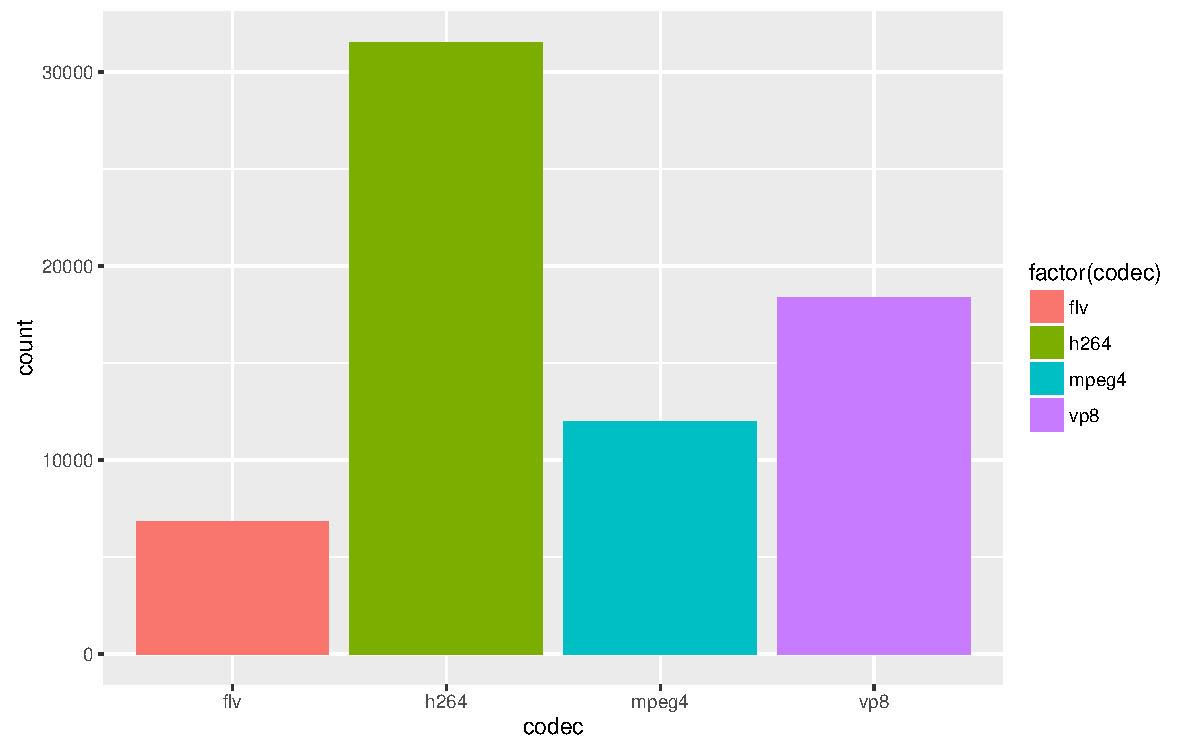
\includegraphics[width=\textwidth]{codec_hist}
            \caption{Histogram of videos by codec type in the youtube dataset}
            \label{codec_hist}
        \end{figure}
        \begin{figure}[!h]
            \centering
            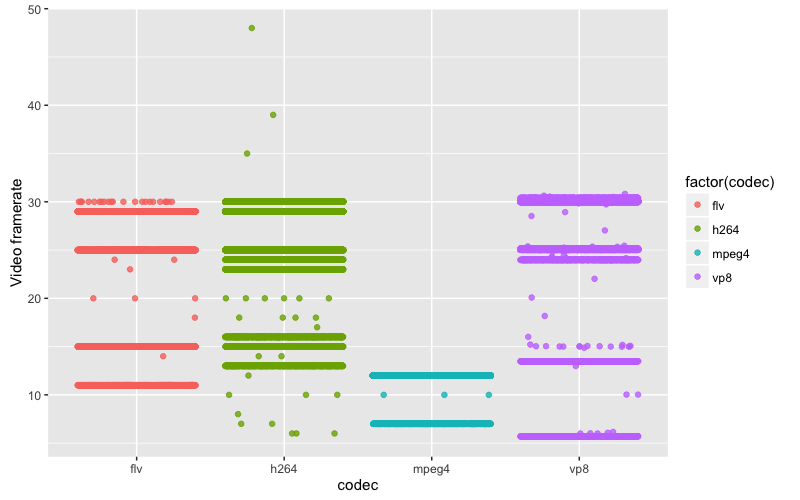
\includegraphics[width=\textwidth]{framerate_hist}
            \caption{Jitter plots of framerates separated by codec type}
            \label{framerate_hist}
        \end{figure}
        \begin{figure}[!h]
            \centering
            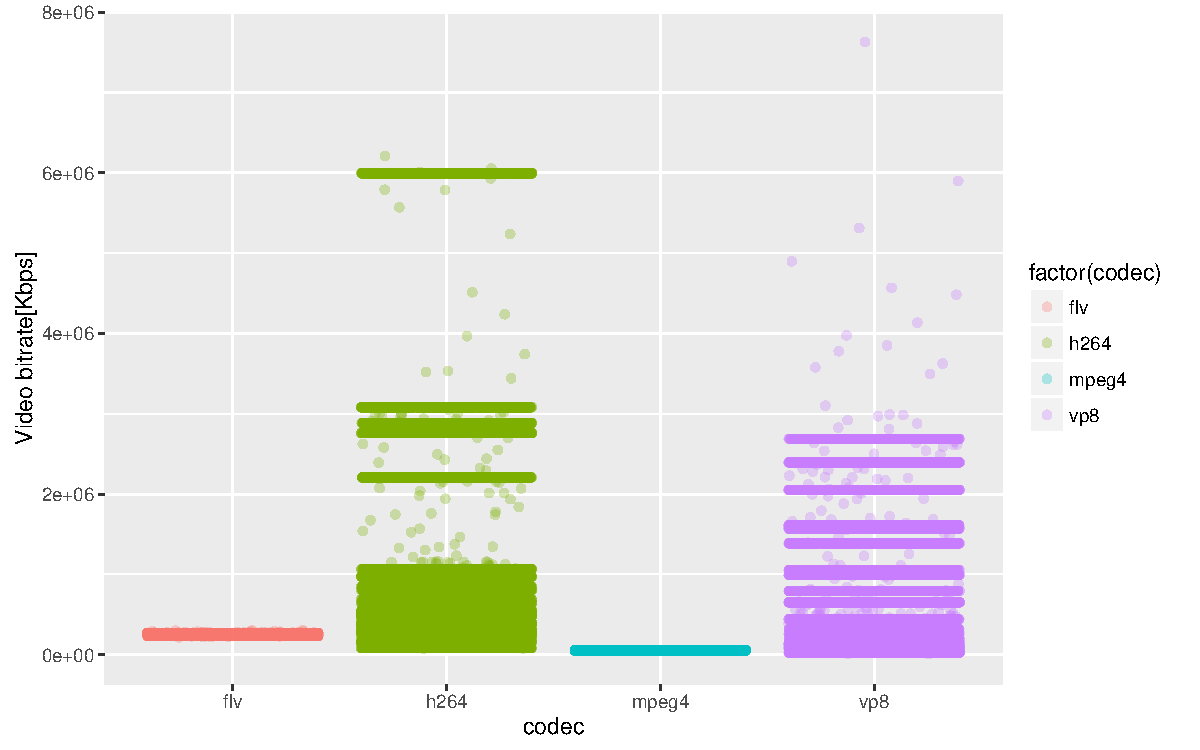
\includegraphics[width=\textwidth]{bitrate_hist}
            \caption{Jitter plots of bitrates separated by codec type}
            \label{bitrate_hist}
        \end{figure}
        \begin{figure}[!h]
            \centering
            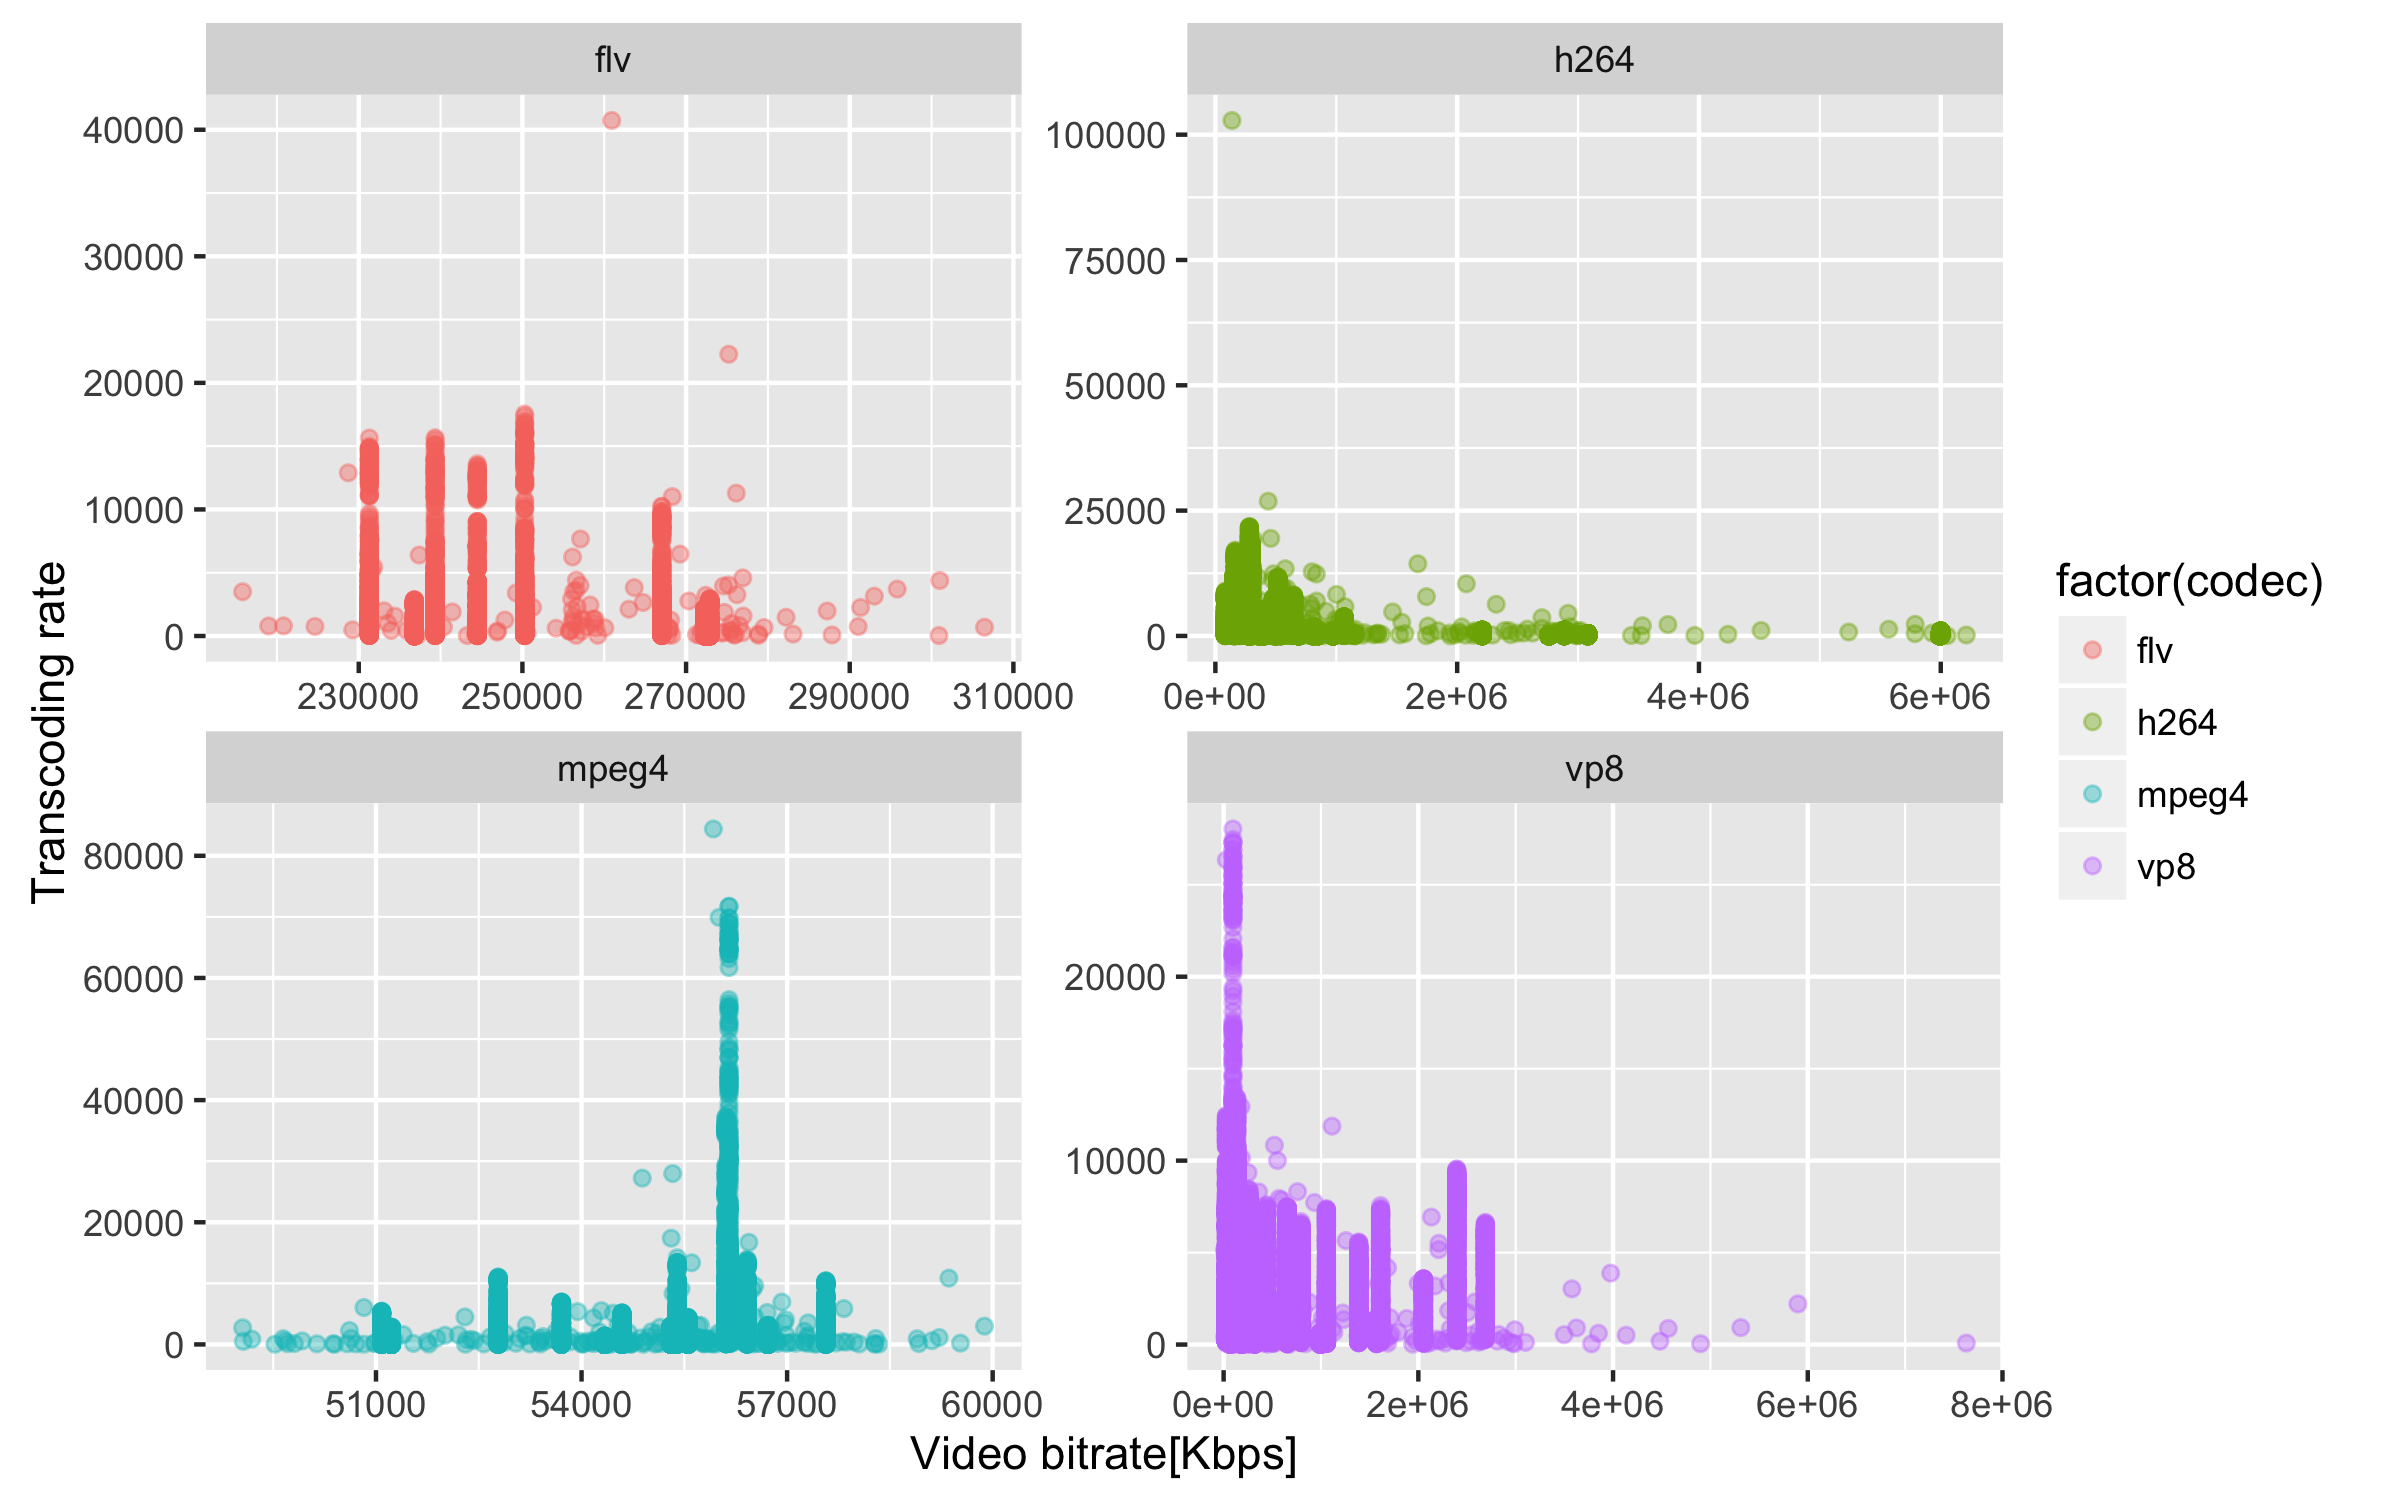
\includegraphics[width=\textwidth]{bitrate_vs_trate}
            \caption{Transcoding rate [fps] v/s video bitrate [Kbps]}
            \label{bitrate_vs_trate}
        \end{figure}
        \begin{figure}[!h]
            \centering
            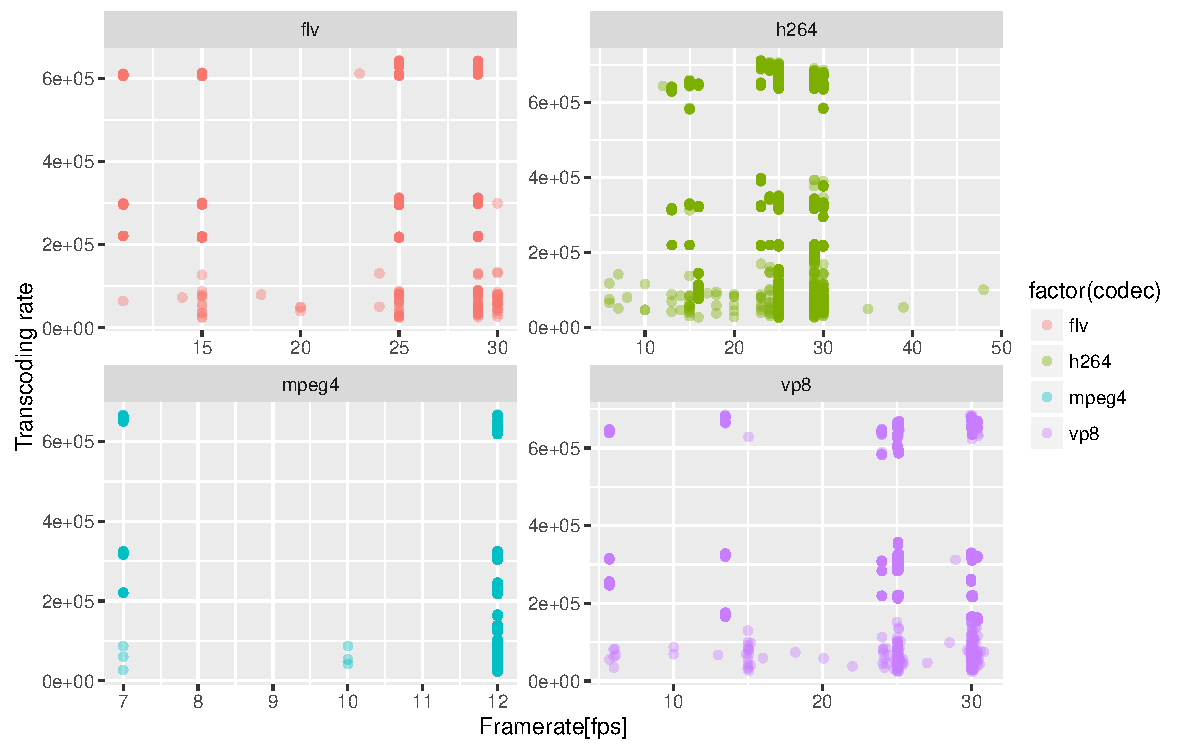
\includegraphics[width=\textwidth]{framerate_vs_trate}
            \caption{Transcoding rate [fps] v/s video framerate [fps]}
            \label{framerate_vs_trate}
        \end{figure}

% B I B L I O G R A P H Y
% -----------------------

% The following statement selects the style to use for references.  It controls the sort order of the entries in the bibliography and also the formatting for the in-text labels.
% \nocite{*}
\bibliographystyle{IEEEtran}
% This specifies the location of the file containing the bibliographic information.  
% It assumes you're using BibTeX (if not, why not?).
\cleardoublepage % This is needed if the book class is used, to place the anchor in the correct page,
                 % because the bibliography will start on its own page.
                 % Use \clearpage instead if the document class uses the "oneside" argument
\phantomsection  % With hyperref package, enables hyperlinking from the table of contents to bibliography             
% The following statement causes the title "References" to be used for the bibliography section:
\renewcommand*{\bibname}{References}

% Add the References to the Table of Contents
\addcontentsline{toc}{chapter}{\textbf{References}}

\bibliography{uw-ethesis}
% Tip 5: You can create multiple .bib files to organize your references. 
% Just list them all in the \bibliogaphy command, separated by commas (no spaces).

% The following statement causes the specified references to be added to the bibliography% even if they were not 
% cited in the text. The asterisk is a wildcard that causes all entries in the bibliographic database to be included (optional).
% \nocite{*}

\end{document}
